\chapter{Methods}
\label{ch:meth}

\noindent In this chapter, we would like to introduce the different methods utilized in our experiments. We will begin in \autoref{sec:single-unit-testbench} with the specification of our initial trials in a simplified \textbdd{single unit} environment, where we could study different reinforcement learning algorithms without the complexity of multiple agents. Next, in \autoref{sec:monolithic-approach} and \autoref{sec:hybrid-approach} we present two different approaches towards multi-agent control, namely \textbdd{monolithic} and \textbdd{hybrid} architectures. The section on the \textbdd{hybrid approach} also contains the definition of our novel \textbdd{trajectory separation} technique.

\section{Single Unit Testbench}
\label{sec:single-unit-testbench}

\noindent We started with a benchmarking study to assess the performance of various RL algorithms within a standardized environment to identify the optimal algorithm for our purposes. We utilized \textbdd{OpenAI's Gym} (not Gymnasium at the time) package (\textcolor{deepblue}{\cite{1606.01540}}) for compatibility with the Lux package and \textbdd{PettingZoo} (\textcolor{deepblue}{\cite{terry2021pettingzoo}}) for environment parallelization. To access state-of-the-art RL algorithms, we conducted our simple benchmarking study using \textbdd{Stable Baselines 3} (\textcolor{deepblue}{\cite{stable-baselines3}}), a reliable collection of reinforcement learning algorithms implemented in \textbdd{PyTorch}. This toolkit provided us with a unified framework for all included algorithms and offered subprocess-level vectorization through Python's \textbdd{Ray} (Ray/RLlib) framework (\textcolor{deepblue}{\cite{moritz2018ray}}), \textbdd{TensorBoard} support (\textcolor{deepblue}{\cite{abadi2016tensorflow}}), and easy out-of-the-box usability. Another significant advantage of Stable Baselines 3 is the fidelity of its implementation to the original specifications in the respective research papers, which meant that only minimal parameter adjustments were necessary for usage. Due to hardware constraints, specifically the availability of only eight logical CPU cores on our local machine, we were limited to running a maximum of eight parallel environments through subprocess-level vectorization.


\subsection{Heuristic Bidding and Factory Placement}
\label{subsec:single-bidding-factory}

\noindent For our testbench, we simplified the problem space to focus on a \textbdd{single-unit scenario}. This involved implementing a straightforward factory placement policy, a basic bidding system, and a simplified controller and action space for our agent. We also employed substantial \textbdd{reward shaping} to focus the agent's learning on a specific task, which was then used for evaluation.

\bigskip 

\noindent The factory placement policy utilized a comprehensive \textbdd{heuristic search} for simplicity, gathering potential spawn positions and identifying areas with high Ice presence. By searching through the ideal locations iteratively, the policy strategically positioned the factory adjacent to Ice clusters within a $3 \times 3$ grid. To completely remove the impact of bidding dynamics in adversarial settings, we adopted a strategy of bidding the minimum required resources while ensuring the opposing agent bid zero. This approach guaranteed us that we started factory placement with the maximum amount of resources possible \protect\footnotemark.

\footnotetext{Our goal was to neutralize the competitive element of the game for this benchmarking study, focusing instead on assessing algorithms through their proficiency in exploration and resource gathering rather than their ability to outperform an adversary.}


\subsection{Actions}
\label{subsec:single-environment}

\noindent In our study, we simplified the game dynamics by converting the factory into a non-learning, heuristic entity. It produced a single Heavy unit at the start of the episode, after which it played no further role, effectively circumventing complications associated with varying entity counts in reinforcement learning settings. Furthermore, we disabled the construction of Lichen, as its contribution to performance metrics — the agent's efficiency in exploring the map and securing necessary resources for the factory — was negligible. Here, therefore, when we use the term \textbdd{agent}, we specifically mean the policy used by the Heavy unit present on the map. This approach, by confining our action space to a singular Discrete action space for one unit, made integration with Stable Baselines 3 easier by ensuring a consistent, discrete-variable-only action space.

\begin{figure}[htbp]
    \centering
    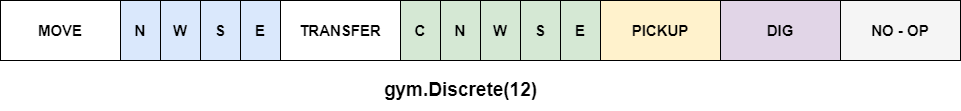
\includegraphics[width=1\linewidth]{images/methods_singleunit/action/controller.png}
    \captionsetup{justification=justified, singlelinecheck=false, width=1\linewidth, labelfont=bf} 
    \caption[]{The action space inside our controller included movements in four cardinal directions, transfers to four cardinal directions and center \protect\footnotemark, pickup \protect\footnotemark, digging, and a no-operation action for debugging.}
    \label{fig:controller}
\end{figure}

\footnotetext{Transfer amount was set to the maximum available resource in cargo, circumventing binning or continuous bounded variables.}
\footnotetext{The same rule applied here as in the previous footnote.}

\noindent \textcolor{deepblue}{\autoref{fig:controller}} illustrates the action space adopted for our benchmarking analysis. We excluded certain operations available in the engine, including self-destruct, recharge, action queues (planning), and the transfer of resources other than Ice. The chosen action needed to be formatted to meet the specifications required by the Lux Engine, as detailed in \textcolor{deepblue}{\autoref{fig:lux-actions_ex}}.

\subsection{Observation}
\label{subsec:single-observation}

\noindent Our observation feature space was also designed with simplicity in mind, consisting of only a one-dimensional vector tailored specifically to the task of Ice mining. We intentionally excluded complex data types such as image maps, text, and extensive global information and conducted a small focused \textbdd{ablation study} to make sure the most significant features are present in the input space of the model. As shown in (\textcolor{deepblue}{\autoref{fig:feature-space}}), the features can be broken down into three components. The first section is the unit vector, which contains information about the state of the agent. Namely, the agent's position, class, team, and cargo data. The other two categories are observations about the environment itself. The features included here are vectors pointing towards the closest factory or ice tiles.

\begin{figure}[htbp]
    \centering
    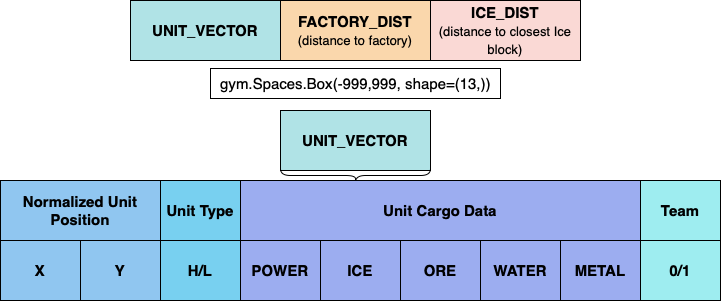
\includegraphics[width=0.8\linewidth]{images/methods_singleunit/observation/feature_space.png}
    \captionsetup{justification=justified, singlelinecheck=false, width=1\linewidth, labelfont=bf} 
    \caption[]{The feature space specifically optimized to maximize Ice collection.}
    \label{fig:feature-space}
\end{figure}

\subsection{Network Architecture}
\label{subsec:single-network}

\noindent Our neural network architecture was also designed with efficient computation and speed in mind, incorporating a small \textbdd{multilayer perceptron (MLP)} with two hidden layers. Each layer uses one \textbdd{linear projection} followed by a \textbdd{ReLU nonlinearity}. The final output layer is a linear projection that maps to the action space of the environment. We evaluated eight state-of-the-art reinforcement learning algorithms: ARS, A2C, DQN, PPO, QR-DQN, R-PPO, TRPO, and MPPO, each utilizing distinct learning approaches and objectives for the agent. Some algorithms employ an actor-critic approach with distinct policy and value heads learned concurrently, while algorithms like DQN and QR-DQN focus on trying to estimate Q-values in different ways for state-action pairs. In contrast, ARS does not learn values, Q-values, or policies directly.

\bigskip

\noindent On-policy actor-critic algorithms often employ \textbdd{separate feature extractors} for the actor and critic components when utilizing simple network architectures like MLPs. This approach is computationally manageable even with relatively small state spaces and has been shown to yield better results (\textcolor{deepblue}{\cite{andrychowicz2020matters}}). However, for more complex models that require a CNN backbone, a shared network architecture should be used since it enables the sharing of critical features between the actor and critic heads while significantly reducing computational overhead. 

\bigskip

\noindent Value-based methods and ARS utilized \textbdd{shared feature extractors}, as they focused solely on learning only Q-values, quantiles, and policy, without the need for distinct learning objectives such as separate value or policy heads. However, not all value-based methods follow this pattern. For instance, Double Deep Q-Learning (\textcolor{deepblue}{\cite{vanhasselt2015deep}}) employs two distinct networks: a primary online network for continuous learning and decision-making, and a separate target network, which is a clone of the primary network. The target network serves as a stable benchmark and is updated less frequently than the primary network.

\begin{figure}[htbp]
    \centering
    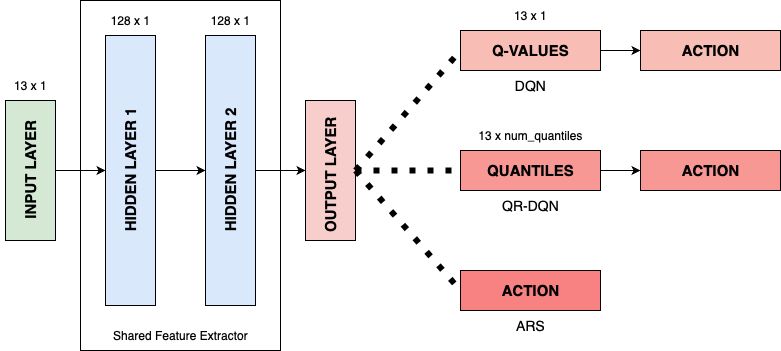
\includegraphics[width=0.8\linewidth]{images/methods_singleunit/net/shared_policy.png}
    \captionsetup{justification=justified, singlelinecheck=false, width=1\linewidth, labelfont=bf} 
    \caption[]{A high-level overview of the neural network layout that employs shared feature extractors used for value-based methods: DQN, QR-DQN, ARS. \protect\footnotemark.}
    \label{fig:shared-policy}
\end{figure}

\begin{figure}[htbp]
    \centering
    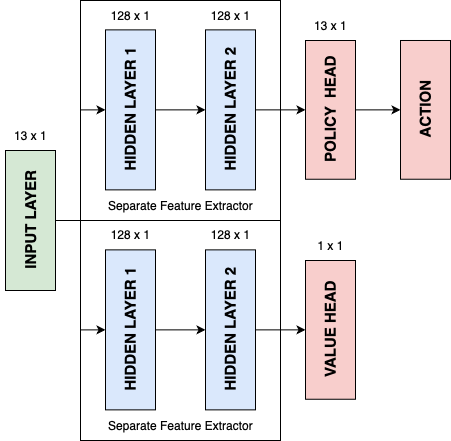
\includegraphics[width=0.5\linewidth]{images/methods_singleunit/net/separate_policy.png}
    \captionsetup{justification=justified, singlelinecheck=false, width=1\linewidth, labelfont=bf} 
    \caption[]{A high-level overview of the neural network layout that employs separate feature extractors used for actor-critic-based methods: A2C, PPO, TRPO, M-PPO, R-PPO. \protect\footnotemark.}
    \label{fig:separate-policy}
\end{figure}

\noindent It is important to note that while Stable Baselines 3 adheres to the specifications outlined in original research papers (\textcolor{deepblue}{\cite{stable-baselines3}}), these documents often omit significant implementation details, necessitating cautious interpretation of results (\textcolor{deepblue}{\cite{shengyi2022the37implementation}}). Moreover, Stable Baselines 3 incorporates significant, occasionally redundant, code overhead. This issue became more apparent when we used a single-file implementation of the PPO algorithm (\textcolor{deepblue}{\cite{huang2022cleanrl}}), to which we introduced several optimization techniques. For this benchmark study, we are continuing with the SB3 baselines.

\footnotetext{It's important to note that in our implementation of Recurrent Proximal Policy Optimization (R-PPO), we opted for two LSTM layers with a hidden size of 128, instead of using traditional linear projection layers due to the recurrent nature of the algorithm.}

\subsection{Reward Function}
\label{subsec:single-reward}

\noindent Lastly, our reward system was designed with heavy shaping to incentivize two specific behaviors. It encouraged the agent to increase Ice collection and motivated the factory to produce more Water than in the previous round. \textbdd{This 1-step lookback} update-based reward system proved to be an effective method for encouraging targeted behaviors within our model.


\begin{equation}
    r_t = \frac{\Delta \text{ } ice\_dug}{100 + \Delta \text{ } water\_produced}
    \label{eq:reward-function}
\end{equation}

\subsection{Trust Region Policy Optimization (TRPO)}
\label{sec:trpo}

\noindent Policy optimization techniques aim to make significant updates to the policy, but this approach has inherent limitations. Specifically, Vanilla Policy Gradient (VPG) methods lack regularization mechanisms, gradient clipping, or specific thresholds for policy updates (\textcolor{deepblue}{\cite{SpinningUp2018}}). This absence often results in a phenomenon known as policy collapse, primarily due to the high variance typically associated with policy gradient methods (\textcolor{deepblue}{\cite{dohare2023overcoming}}). In classical neural network architectures, updating the model’s parameters is straightforward because the loss function guides the adjustment of weights based on the deviation from known labels in the training dataset. However, in reinforcement learning, especially in model-free scenarios, this process becomes more complex. There is no explicit ground truth action for each state; instead, weight adjustments are guided by reward signals, which are often sparse and delayed, making it challenging to directly correlate actions to desired outcomes. This implies that in almost every deep RL task, there are some updates that push the policy gradients toward suboptimal directions. If such a negative update is relatively large, it can lead to a significant degradation of the policy, a situation from which the algorithm might not recover. This scenario is commonly referred to as \textbdd{policy collapse}.

\bigskip

\noindent Trust Region Policy Optimization (\textcolor{deepblue}{\cite{schulman2017trust}}) was the first among policy gradient methods to implement a hard limit on gradient updates, based on the Kullback-Leibler Divergence between the probability distributions of actions before and after the updates. This constraint ensures that the model's parameters remain close in the parameter space, thus helping the model mitigate potentially detrimental updates. The parameter update rule looks like the following (\textcolor{deepblue}{\cite{schulman2017trust}; \autoref{eq:trpo-update}}):

\begin{equation}
    \theta_{k+1} = \text{arg }\underset{\theta}{\text{max }} L(\theta_k, \theta) \quad \text{w.r.t.} \quad D_{KL}(\theta || \theta_k) \leq \delta,
    \label{eq:trpo-update}
\end{equation}

\noindent where $L(\theta_k, \theta)$ is defined as the \textbdd{surrogate advantage function}, which measures how much better does $\pi_{\theta}$ perform over $\pi_{\theta_k}$ (\textcolor{deepblue}{\cite{schulman2017trust}; \autoref{eq:surrogate-advantage}}).

\begin{equation}
    L(\theta_k, \theta) = \mathbb{\hat{E}}_{s, a \sim \pi_{\theta_k}} \left [ \underbrace{\frac{\pi_{\theta}(a | s)}{\pi_{\theta_k}(a | s)}}_{\text{importance sampling ratio}} \hat{A}^{\pi_{\theta_k}}(s, a)\right]
    \label{eq:surrogate-advantage}
\end{equation}

\noindent The update in \textcolor{deepblue}{\autoref{eq:trpo-update}}) is not straightforward to compute in an explicit way. Therefore, TRPO approximates the impact of a small change in policy parameters using a first-order Taylor series expansion. It linearly approximates how the objective function changes with a small change in parameters, constrained by a second-order Taylor expansion of the KL divergence to ensure the change is not too large (\textcolor{deepblue}{\cite{schulman2017trust}; \autoref{eq:trpo-update-approx}}).

\begin{equation}
    \theta_{k+1} = \text{arg }\underset{\theta}{\text{max }} g^T(\theta - \theta_k) \quad \text{w.r.t.} \quad \frac{1}{2}(\theta - \theta_k)^T H(\theta - \theta_k) \leq \delta
    \label{eq:trpo-update-approx}
\end{equation}

\noindent The above optimization problem is addressed using Lagrangian duality (\cite{KnowlesLagrangianDuality}), but potential inaccuracies from the Taylor approximation may not meet the KL divergence constraint, needing for a backtracking line-search for correct updates. Due to the computational intensity of directly calculating and storing the inverse Hessian, the conjugate gradient method (\cite{conjugate}) is employed for approximation.

\begin{algorithm}[htbp]
\caption{Trust Region Policy Optimization (\cite{schulman2017trust})} 
\label{alg:TRPO}

\begin{algorithmic}[1]
\State \textbdd{Input:} Initial parameters for both the value, $\phi_0$, and policy functions, $\theta_0$.
\State \textbdd{Hyperparameters:} KL-divergence threshold, $\delta$, number of backtracks, $K$, and the backtracking coefficient, $\alpha$.
\For { $k = 0, 1, 2, \hdots$ }
    \State Collect rollouts, $D_k$, using current policy $\pi_k$.
    \State Compute the rewards-to-go term $\hat{R_t}$. 
    \State Estimate the advantage function, $\hat{A_t}$, using any general advantage estimator.
    \State Calculate the policy gradient based on \textcolor{deepblue}{\autoref{eq:policy-gradient-sample}}.
    \State Utilize the conjugate gradient method to calculate:
    \begin{equation*}
    \hat{x_k} \approx \hat{H}^{-1}_{k} \hat{g_k}
    \end{equation*}
    \State Use backtracking line search to update the policy:
    \begin{equation*}
    \theta_{k+1} = \theta_k + \alpha^j \sqrt{\frac{2\delta}{\hat{x_k^T} \hat{H_k} \hat{x_k}}} \hat{x_k} 
    \end{equation*}
    \text{\hspace{18pt}where $j$ is the smallest possible integer value that satisfies the KL constraint.}
    \State Approximate the value function $V_{\phi}(s_t)$ by mean-squared error:
    \begin{equation*}
    \phi_{k+1} = \arg \min_{\phi} \frac{1}{|D_k| T} \sum_{\tau \in D_k} \sum_{t=0}^{T} \left( V_\phi(s_t) - \hat{R_t} \right)^2
    \end{equation*}
    \text{\hspace{18pt} via a gradient descent algorithm.}
\EndFor
\end{algorithmic}
\end{algorithm}


\subsection{Advantage Actor Critic (A2C)}
\label{sec:a2c}

\noindent The Advantage Actor-Critic is a family of algorithms, including Asynchronous Advantage Actor Critic (A3C) and Advantage Actor Critic (A2C), and were developed by the Deepming team at Google (\textcolor{deepblue}{\cite{mnih2016asynchronous}}). A3C employs multiple parallel actor-learners that asynchronously update a global network, introduced one year after Trust Region Policy Optimization (TRPO). A3C, notable for its asynchronicity, employed \textbdd{fixed-length episode segments} for both updates and advantage function calculations and it also utilized a shared feature extractor for the value and policy heads. As a highly influential algorithm at its time, A3C underwent extensive benchmarking across various Gym environments. These tests aimed to determine whether its asynchronous nature genuinely enhanced performance or if apparent improvements were due to unrelated factors, such as optimal hyperparameter settings or variability introduced by initialization and seeding techniques. One year after A3C's release, OpenAI conducted a comprehensive benchmark study on A3C, its synchronous counterpart A2C, and the ACKTR algorithms (\textcolor{deepblue}{\cite{wu2017scalable}}). The study concluded that the asynchronicity and the associated noise did not enhance the performance of A3C. Surprisingly, it was found that A2C, which employs the same architecture but synchronizes \textbdd{actor-learner} updates to a global network, performed comparably to A3C. Notably, in A2C, the actor-learners wait for each other and update the central network by averaging over the learners, a process that benefits from GPU parallelization. This contrasts with the original design of A3C, which was optimized for running on CPU threads to accelerate training.

\bigskip

\noindent The Advantage Actor Critic (A2C) algorithm computes its loss function using the advantage function, necessitating estimates of both state values and state-action values (\textcolor{deepblue}{\autoref{eq:advantage}}). This requirement may seem atypical as it implies the need for separate networks: one to estimate state values and another for action-value estimations. 

\begin{equation}
    L^{A2C}(\theta) = \mathbb{\hat{E}}_{t} \left [ \text{log } \pi_{\theta}(a_t | s_t) \hat{A}_t \right]
    \label{eq:a2c-update}
\end{equation}

\noindent From (\textcolor{deepblue}{\cite{mnih2016asynchronous}; \autoref{eq:a2c-update}}), it is clear that the advantage function, $\hat{A}_t$ is simply an approximation of the actual true advantage. However, this can be reformulated to include only the value functions, using the Bellman Equations (\textcolor{deepblue}{\autoref{eq:bellman-action-value}}). According to these equations, the expected return of taking action $a_t$ in state $s_t$ can be broken down into the immediate reward $r_{t+1}$ plus the discounted future returns, as estimated by the value function $V^{\pi}_{\phi}$ at the subsequent state $s(t+1)$ (\textcolor{deepblue}{\cite{mnih2016asynchronous}; \autoref{eq:a2c-advantage-estimation}}). 

\begin{equation}
    \hat{A}^{\pi}(s_t, a_t) = r(s_{t+1}, a_{t+1}) + \gamma V^{\pi}_{\phi}(s_{t+1}) - V^{\pi}_{\phi}(s_{t})
    \label{eq:a2c-advantage-estimation}
\end{equation}

\noindent The seminal A2C paper also introduced n-step Actor-Critic learning, which updates both the policy and the value function using an \textbdd{n-step lookahead}. This method complicates advantage estimation by requiring the calculation of the Temporal Difference \textbdd{(TD) target}, $r(s_{t+1}, a_{t+1}) + \gamma V^{\pi}_{\phi}(s_{t+1})$, across $n$ steps, from which the value of the state, at timestep $t$, under policy $\pi$, parameterized by $\phi$ is subtracted (\textcolor{deepblue}{\cite{mnih2016asynchronous}; \autoref{eq:a2c-advantage-estimation-n-step}}).

\begin{equation}
    \hat{A}^{\pi}(s_t, a_t) = \underbrace{{\sum_{i=0}^{n-1}} \left (\gamma^i r(s_{t+i}, a_{t+i}) + \gamma^n V^{\pi}_{\phi}(s_{t+n}) \right )}_{\text{n-step return}} - V^{\pi}_{\phi}(s_{t})
    \label{eq:a2c-advantage-estimation-n-step}
\end{equation}

\noindent In the official paper, the value head of the network, characterized as an n-to-1 linear projection connected to a CNN backbone is updated by minimizing the squared difference between the bootstrapped n-step return and the predicted value, which helps approximate $V_{\phi}(s_t)$ (\textcolor{deepblue}{\cite{mnih2016asynchronous}; \autoref{eq:a2c-value-optimization}}).

\begin{equation}
    \phi_{k+1} = \arg \min_{\phi} \frac{1}{2} \sum_{t=0}^{T} \left( V_\phi(s_t) - \hat{R_t} \right)^2
    \label{eq:a2c-value-optimization}
\end{equation}


\noindent Additionally, as a method of regularization, entropy is added to the policy $\pi$ to enhance exploration rates, a technique shown to improve performance during exploration phases (\textcolor{deepblue}{\cite{penge}}). 

\begin{equation}
    \nabla_{\theta} L^{A2C}(\theta, \phi) = \hat{\mathbb{E}}_{t} \left [ \nabla_{\theta}\log \pi_{\theta}(a_t | s_t) (R_t - V_{\phi}(s_t)) + \underbrace{\beta \nabla_{\theta} H(\pi_{\theta}(s_t))}_{\text{entropy}} \right]
    \label{eq:a2c-gradient-calculation}
\end{equation}

\noindent As detailed in \textcolor{deepblue}{\cite{mnih2016asynchronous}; \autoref{eq:a2c-advantage-estimation-n-step}}, the final gradient calculation for the policy head enables us to optimize of parameters of the policy, $\theta$, using various techniques, including SGD, RMSProp or Adam.

\begin{algorithm}[htbp]
\caption{Advantage Actor Critic (A2C) - One Actor (\cite{mnih2016asynchronous})} 
\label{alg:A2C}

\begin{algorithmic}[1]
\State \textbdd{Input:} Initial parameters for both the value, $\phi_0$, and policy functions, $\theta_0$.
\State \textbdd{Hyperparameters:} Number of lookahead steps, $n$, the strength of the entropy, $\beta$, and the global shared counter, $T$.

\Repeat
    \State Set back gradients to 0.
    \State Synchronize thread-specific parameters for correct global updates.
    \State Set thread step counter, $t$, to 1.
    \Repeat
        \State Perform action according to current policy $\pi_{\theta}(a_t \mid s_t)$ and receive reward $r_t$
        \State $t = t + 1$
        \State $T = T + 1$
    \Until current state is terminal or $t_{max}$ is reached.
    \If{state is terminal}
        \State $R = 0$
    \Else
        \State $R = V_{\phi}(s_t)$
    \EndIf
    \For{$i = \{t-1, \hdots,  t_{\text{start}}\}$}
        \State $R = r_i + \gamma R$
        \State Accumulate gradients using \textcolor{deepblue}{\autoref{eq:a2c-value-optimization}}.
        \State Accumulate gradients of \textcolor{deepblue}{\autoref{eq:a2c-gradient-calculation}} using SGD or RMSProp.
    \EndFor
    \State Perform asynchronous update of both $\theta$ and $\phi$.
\Until{$T > T_{\max}$}
\end{algorithmic}
\end{algorithm}

\bigskip

\noindent 
Interestingly, Proximal Policy Optimization (PPO) performs similarly to A2C when limited to a single training epoch (\textcolor{deepblue}{\cite{huang2022a2c}}). In this setting, $\pi_{\theta_{old}}$ and $\pi_{\theta}$ remain unchanged during the epoch, which means the clipping operation, a key feature in PPO's loss calculation, does not fire. As a result, PPO's loss function becomes identical to that of A2C, leading to the same gradient if the data input is the same. 
However, this observation should be taken with a grain of salt. In practical implementations, achieving perfect determinism in the code to ensure log ratios equal one is impossible.


\subsection{Proximal Policy Optimization (PPO)}
\label{sec:ppo}

\noindent Proximal Policy Optimization extends the principles established by TRPO, with the aim of maximizing the magnitude of policy updates while ensuring they remain under certain controlled limits (\textcolor{deepblue}{\cite{schulman2017proximal}}). PPO distinguishes itself from TRPO by moving away from the use of hard KL-divergence constraints and second-order approximation methods, introducing two new approaches for computing policy gradients instead. The first variant, \textbdd{PPO-Penalty}, incorporates a dynamically adjusted KL-divergence penalty coefficient into the objective function, deviating from TRPO's fixed threshold approach. However, despite its flexibility, PPO-Penalty has not demonstrated any performance improvements over TRPO and, thus, will not be further discussed. In subsequent references to PPO, we will specifically refer to the more performant variant, \textbdd{PPO-Clip}. PPO-Clip lacks a KL-divergence term in its objective function and employs a \textbdd{clipping mechanism} that effectively limits the distance between old and updated policies.

\bigskip

\noindent PPO-Clip updates its policy using a formulation similar to that in \textcolor{deepblue}{\autoref{eq:trpo-update}}, where the loss function employs a surrogate advantage function represented by the ratio $r_t(\theta, \theta_k)$. This ratio, commonly referred to as the importance sampling ratio in the literature, measures the improvement of the current updated policy over the old policy. By applying this formulation to the TRPO loss function, (\textcolor{deepblue}{\cite{schulman2017proximal}; \autoref{eq:surrogate-advantage}}), we get the following equation:

\begin{equation}
    L^{PPO}(\theta_k, \theta) = \mathbb{\hat{E}}_{s, a \sim \pi_{\theta_k}} \left [ r_t(\theta) \hat{A}^{\pi_{\theta_k}}(s, a)\right]
    \label{eq:PPO-loss}
\end{equation}


\noindent Without constraints, this loss function results in excessively large policy updates. To address this, PPO-Clip incorporates a \textbdd{clipping mechanism} on the probability ratio (\textcolor{deepblue}{\cite{schulman2017proximal}; \autoref{eq:PPO-loss-clipped}}) \protect\footnotemark.

\begin{equation}
    L^{PPO}(\theta_k, \theta) = \mathbb{\hat{E}}_{s, a \sim \pi_{\theta_k}} \left [ \text{min}(r_t(\theta, \theta_k) \hat{A}^{\pi_{\theta_k}}(s, a),\text{ clip}(r_t(\theta, \theta_k), 1-\epsilon, 1+\epsilon)\hat{A}^{\pi_{\theta_k}}(s, a)\right]
    \label{eq:PPO-loss-clipped}
\end{equation}

\footnotetext{It should be noted that the final objective function of PPO also incorporates an entropy term, $H(\pi_{\theta}(s_t))$, to increase exploration.}

\noindent This complex- and daunting-looking loss function is surprisingly simple while effectively limiting the magnitude of policy updates in PPO-Clip. The first term within the empirical estimate is derived from the original loss functions used in both PPO and TRPO (\textcolor{deepblue}{\cite{schulman2017proximal}; \autoref{eq:PPO-loss}}), incorporating a modification to the surrogate objective function. The clipping mechanism limits the importance sampling ratio to the interval [$1-\epsilon, 1+\epsilon$]. If the ratio exceeds these bounds, it is clipped and then multiplied by the advantage estimate, calculated using methods from TRPO and A2C that involve the Bellman Equations and n-step returns (\textcolor{deepblue}{\autoref{eq:a2c-advantage-estimation-n-step}}). The min operation at the end establishes a conservative lower bound on the unclipped objective, effectively ignoring improvements in the probability ratio that would enhance the objective and only incorporating changes that would degrade it. There is a more intuitive approach to the loss function that simplifies the concept and helps build an understanding of the clipping mechanism (\textcolor{deepblue}{\cite{SpinningUp2018}; \cite{schulman2017proximal}; \autoref{eq:PPO-loss-clipped-simplified}}):

\begin{equation}
    L^{PPO}(\theta_k, \theta) = \mathbb{\hat{E}}_{s, a \sim \pi_{\theta_k}} \left [ \text{min}(r_t(\theta, \theta_k) \hat{A}^{\pi_{\theta_k}}(s, a)\text{, }g(\epsilon, \hat{A}^{\pi_{\theta_k}}(s, a))\right],
    \label{eq:PPO-loss-clipped-simplified}
\end{equation}

\noindent where $g$ takes the following form (\textcolor{deepblue}{\cite{SpinningUp2018}; \cite{schulman2017proximal}; \autoref{eq:PPO-gfunction}}):

\begin{equation}
    g(\epsilon, \hat{A}) = 
        \begin{cases} 
        (1 + \epsilon)\hat{A} & \text{if } \hat{A} \geq 0 \\
        (1 - \epsilon)\hat{A} & \text{if } \hat{A} < 0 
        \end{cases}
    \label{eq:PPO-gfunction}
\end{equation}

\noindent When examining the case where the advantage estimate is positive, the term $g$ becomes $(1+\epsilon)\hat{A}$, suggesting that the advantage supports a positive direction in the surrogate objective. Since $\hat{A}$ appears in both terms within the \textbdd{min} function, we can factor it out, simplifying the expression to: $\min(r_t(\theta, \theta_k), (1+\epsilon))$. This indicates that if $\pi_{\theta}(a|s)$ exceeds $(1+\epsilon)\pi_{\theta_k}(a|s)$, the \textbdd{min} function fires, adding a ceiling of $(1+\epsilon)\hat{A}$ on the policy update. Similarly, if the advantage estimate $\hat{A}$ is negative, the objective will only increase if the selected action becomes less likely in the future, meaning a decrease in $\pi_{\theta}(a|s)$. When factoring out the negative advantage estimate, care must be taken due to the negative sign inside $(1-\epsilon)$. This detail converts the \textbdd{min} function to a \textbdd{max} function. This change imposes a ceiling of \( (1-\epsilon)\hat{A} \) on the policy updates, effectively limiting how much the policy can adjust in response to actions that degrade the final objective.

\bigskip

\noindent Surprisingly, heavily adopted implementations of PPO integrate both clipping mechanisms and KL-Divergence thresholds to maintain controlled policy updates (\textcolor{deepblue}{\cite{shengyi2022the37implementation}}). It has been demonstrated in various instances that clipping alone is insufficient to limit excessive updates to the model (\textcolor{deepblue}{\cite{stable-baselines-issue213}}). If the KL-Divergence exceeds a predefined limit, the update process is stopped early. In practice, PPO utilizes \textbdd{fixed-length trajectory segments}, where a single learner collects a specified number of steps ($N$) in multiple environments ($M$) before proceeding to update the model. This structured approach categorizes the learning process into two parts: a \textbdd{rollout phase} and a \textbdd{learning phase}. For updates, PPO utilizes \textbdd{minibatches} randomly sampled from the rollout batch, allowing certain steps to be sampled multiple times. Additional implementation details, not specified in the seminal paper, include the necessity for clipping the value function as well (\textcolor{deepblue}{\cite{Engstrom2020Implementation}}) and the application of \textbdd{clip range annealing}, similar to learning rate annealing. 

\begin{algorithm}[htbp]
\caption{PPO-Clip (\cite{schulman2017proximal})} 
\label{alg:PPO-Clip}

\begin{algorithmic}[1]
\State \textbdd{Input:} Initial parameters for both the value, $\phi_0$, and policy functions, $\theta_0$.
\State \textbdd{Hyperparameters:} KL-divergence threshold, $\delta$, and the clip threshold, $\epsilon$.
\For { $k = 0, 1, 2, \hdots$ }
    \State Collect rollouts, $D_k$, using current policy $\pi_k$.
    \State Compute the rewards-to-go term $\hat{R_t}$. 
    \State Estimate the advantage function, $\hat{A_t}$, using any general advantage estimator.
    \State Update the policy by maximizing the clipped PPO objective: 
    \begin{equation*}
    \theta_{k+1} = \arg \max_{\theta} \frac{1}{|D_k| T} \sum_{\tau \in D_k} \sum_{t=0}^{T} \text{min}\left (r_t(\theta, \theta_k) \hat{A}^{\pi_{\theta_k}}(s_t, a_t)\text{, }g(\epsilon, \hat{A}^{\pi_{\theta_k}}(s_t, a_t)\right),
    \end{equation*}
    \text{\hspace{16pt} using optimization techniques such as SGD, RMSProp, or Adam.}
    \State Approximate the value function $V_{\phi}(s_t)$ by mean-squared error:
    \begin{equation*}
    \phi_{k+1} = \arg \min_{\phi} \frac{1}{|D_k| T} \sum_{\tau \in D_k} \sum_{t=0}^{T} \left( V_\phi(s_t) - \hat{R_t} \right)^2
    \end{equation*}
    \text{\hspace{16pt} via a gradient descent algorithm.}
\EndFor
\end{algorithmic}
\end{algorithm}

\subsection{Recurrent Proximal Policy Optimization (R-PPO)}
\label{sec:rppo}

\noindent R-PPO (\textcolor{deepblue}{\cite{pleines2022generalization}; \cite{stable-baselines3}}), a recurrent variant of the Proximal Policy Optimization (PPO) algorithm, integrates \textbdd{LSTM layers} to establish a recurrent policy framework. This enables the policy to consider not only the current state but also the historical information from the agent’s past interactions, encapsulated in the hidden state $h_t$ at each timestep. This adaptation makes the action selection at each timestep dependent on both the state $s_t$ and $h_t$. This architecture is particularly advantageous in environments characterized by partial observability, or \textbdd{Partially Observable Markov Decision Processes (POMDPs)}, where the recurrent nature allows the policy to access a more extensive portion of the observational history from an experience replay. Additionally, R-PPO is well-suited for longer or continuous tasks that are not episodic, as recurrence can capture \textbdd{temporal dependencies} across extended periods. Recurrence was not initially introduced in policy gradient methods but was first explored in Deep Q-Networks (DQN) (\textcolor{deepblue}{\cite{andrychowicz2021what}}). These networks experimented with the ways in which episodes and their corresponding hidden states are sampled from an experience replay buffer.

\bigskip

\noindent In terms of implementation, most approaches (\textcolor{deepblue}{\cite{shengyi2022the37implementation}}) employ a convolutional neural network backbone linked to an LSTM or a dual-stream transformer. The outputs are then processed through either shared or separate feature extractors for the value and policy heads of the PPO. Some implementations also feature a shared linear layer before diverging into two distinct extractors. The loss functions of PPO and its recurrent variant, R-PPO, are largely similar, with a key difference in the importance sampling ratio. In R-PPO, both $\pi_{\theta}$ and $\pi_{\theta_k}$ depend on the hidden state of the recurrent layer, expressed as: $\pi_{\theta}(a_t | s_t, h_t)$ (\textcolor{deepblue}{\cite{pleines2022generalization}; \autoref{eq:R-PPO-ration}}).

\begin{equation}
    r_t(\theta, \theta_k) = \frac{\pi_{\theta}(a_t | s_t, h_t)}{\pi_{\theta_k}(a_t | s_t, h_t)}
    \label{eq:R-PPO-ration}
\end{equation}

\noindent Incorporating LSTM layers into a model significantly modifies the processing of rollout data, modifies the loss function (\textcolor{deepblue}{\cite{pleines2022generalization}; \autoref{eq:R-PPO-ration}}), and requires adjustments to the forward pass. Unlike the original PPO, which processes minibatches of potentially truncated data from the rollout buffer due to predetermined trajectory lengths, LSTM necessitates orderly processing of sequences to maintain temporal dependencies (\textcolor{deepblue}{\cite{shengyi2022the37implementation}}). This requires that rollout data be segmented into episodes, which are then divided into smaller sequences of fixed lengths. Given that episode lengths are different, maintaining a fixed \textbdd{sequence length}, unless it matches the lengths of episodes, can lead to padding shorter episodes with many zero-filled steps. This padding introduces substantial noise into the LSTM's input sequences, complicating the learning process and necessitating a masking procedure for loss calculation.

\bigskip

\noindent Correctly managing the hidden state is crucial when incorporating LSTMs into a model. The output hidden state from one sequence must serve as the input hidden state for the subsequent sequence, a process known as \textbdd{truncated backpropagation through time} (\textcolor{deepblue}{\cite{tallec2017unbiasing}}). Additionally, it is more efficient to process the entire batch of data through the network's backbone before segmenting it for the LSTM layers. After processing through the recurrent layers, the data must be reshaped once again to feed into the final linear projection layers for both the policy and value heads.

\bigskip

\noindent There is an ongoing debate about the benefits of refreshing advantages and hidden states before each minibatch epoch in policy gradient methods. Research indicates that recalculating advantage estimates prior to each epoch can significantly enhance the performance of these methods (\textcolor{deepblue}{\cite{andrychowicz2021what}}). Similarly, studies suggest that updating hidden states before collecting experiences and recalculating them before each minibatch epoch can notably improve the performance of R-PPO (\textcolor{deepblue}{\cite{kapturowski2018recurrent}; \cite{GuptaRecurrentPPO}}). However, other sources contend that recalculating advantages before every minibatch epoch does not yield substantial improvements (\textcolor{deepblue}{\cite{pleines2022generalization}}).

\subsection{Masked Proximal Policy Optimization (M-PPO)}
\label{subsec:M-PPO}

\noindent \textbdd{Action masking} is a significantly underutilized tool in Reinforcement Learning that enables a learning agent to avoid sampling invalid actions from the action space distribution (\textcolor{deepblue}{\cite{Huang_2022}}). These invalid actions, determined by the constraints of the environment, can significantly reduce the effective size of the action space. For example, OpenAI's Dota AI (\textcolor{deepblue}{\cite{openai2019dota}}) operates within an action space that has over 1.8 million dimensions, where a substantial number of actions—such as moving to invalid spaces, buying items without sufficient in-game currency, or using spells without the required resources—are infeasible. Action masking can effectively reduce this to a small fraction. Despite its simplicity, action masking is rarely discussed in academic literature, with only a few seminal papers addressing it (\textcolor{deepblue}{\cite{vinyals2017starcraft}; \cite{malmo}}). Invalid action masking produces a valid policy gradient in policy optimization methods.

\bigskip

\noindent Invalid action masking can be implemented through various methods, each differing in scalability and effectiveness (\textcolor{deepblue}{\cite{SpinningUp2018}}). One approach is to assign \textbdd{negative penalties} to invalid actions, which can exponentially increase the hyperparameter space with the number of invalid actions. This method typically yields unfeasible reward shaping requirements and is generally not recommended (\textcolor{deepblue}{\cite{app13148283}; \cite{dietterich1999hierarchical}}). More efficient techniques include \textbdd{true} and \textbdd{naive invalid action masking}, which directly prevent the selection of infeasible actions, improving the sample efficiency of an RL algorithm. 

\bigskip

\noindent The former operates by modifying the output logits of infeasible actions before converting these logits into a probability distribution from which actions are sampled. Specifically, the logits for invalid actions are set to an extremely large negative value (\textcolor{deepblue}{\autoref{fig:invalid-action-masking}}), effectively causing the softmax function to assign a near-zero probability to these actions (\textcolor{deepblue}{\cite{Huang_2022}}). However, this approach should be approached with caution due to potential issues with seeding and different implementations of categorical distributions in PyTorch or Tensorflow and inherent numerical uncertainties, which can result in this process not being entirely deterministic in masking out actions. The naive invalid action masking method employs a renormalized policy that ensures no invalid action can be chosen. However, it updates the gradient based on the unnormalized policy, which still includes the invalid actions. This method is termed "naive" because it does not alter the logit values of invalid actions; instead, it simply renormalizes the probabilities across the valid actions in the policy.

\bigskip

\begin{figure}[htbp]
    \centering
    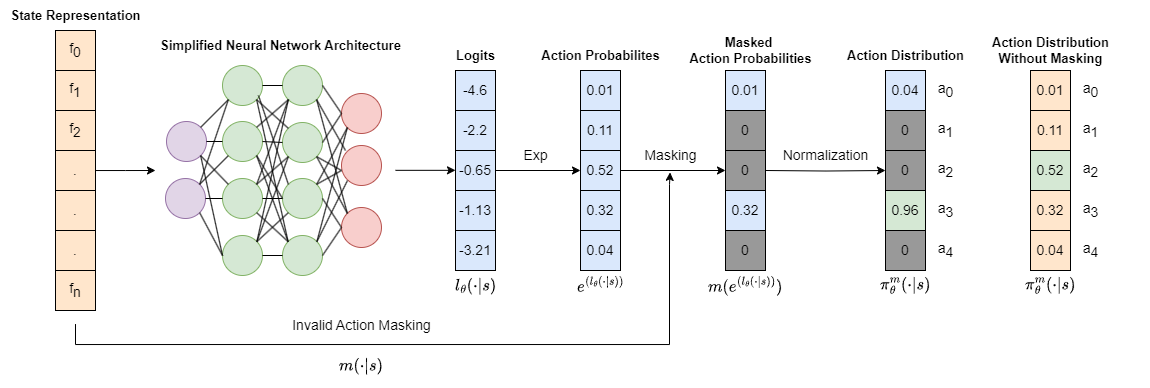
\includegraphics[width=1\linewidth]{images/methods_algos/m_ppo/invalidactionmasking.png}
    \captionsetup{justification=justified, singlelinecheck=false, width=1\linewidth, labelfont=bf} 
    \caption[]{A high-level overview of how invalid action masking affects the final action distribution. Note that logits here represent the log probabilities of actions and are sent through a masking procedure where invalid actions are filtered out. After masking, exponentiation is applied to convert these log probabilities back into raw probabilities. Subsequently, normalization is performed to transform these probabilities into a valid probability distribution.}
    \label{fig:invalid-action-masking}
\end{figure}

\noindent Studies have demonstrated that both true and naive invalid action masking methods perform comparably up to a certain point, with minor differences in convergence times (\textcolor{deepblue}{\cite{Huang_2022}}). Convergence is context-specific, typically defined by the learning agent consistently reaching a predetermined performance threshold. However, naive invalid action masking has some drawbacks, such as susceptibility to KL divergence explosion, which can result in significantly larger policy updates compared to true invalid action masking. Additionally, naive invalid action masking is sensitive to increases in environment size; for example, scaling up the size of a grid world map can significantly impair performance.

\bigskip

\noindent Now that we have explored the intricacies behind action masking, what exactly is M-PPO, and how does it function in practice? Simply put, M-PPO modifies the standard PPO algorithm by incorporating \textbdd{domain knowledge} into action selection, thus guiding gradient updates faster towards a global optimum. M-PPO is essentially a straightforward extension of the original PPO algorithm. At first glance, it may seem like a "cheat code," and indeed, it could potentially be used as such. Theoretically, one could build the heuristics behind the invalid action masking within a system to render the algorithm completely deterministic, adhering to a \textbdd{logic-based approach}. However, such modifications are purely hypothetical and would likely hold little practical value or relevance in real-world applications.


\subsection{Deep Q Network (DQN)}
\label{sec:dqn}

\noindent The fundamental concept behind Deep Q-Networks (DQNs) builds on the principles of classical Q-Learning, aiming to estimate the action-value function using the Bellman Equations to ensure convergence through value iteration (\textcolor{deepblue}{\cite{mnih2013playing}; \cite{stable-baselines3}}). However, this approach often struggles in practice due to issues like scalability and limited generalization. Value iteration and Q updates, which rely on sequences of actions in the environment, introduce a temporal sequence bias. This bias persists even in function approximators, whether they are linear or neural networks, that attempt to estimate the action-value function through parameterized approximations. DQNs are trained using neural network function approximators by minimizing a specific loss function (\textcolor{deepblue}{\cite{mnih2013playing}; \autoref{eq:Q-neural-loss}}).

\begin{equation}
    L^{DQN}(\theta_k, \theta) = \mathbb{E}_{s, a \sim \pi_{\theta_k}} \left [ \left (  \mathbb{E}_{s' \sim \epsilon} \left [ r + \gamma \underset{a'}{\text{ max}} Q(s', a' | \theta_k ) \right] - Q(s, a | \theta)  \right )^2\right]
    \label{eq:Q-neural-loss}
\end{equation}


\noindent In Deep Q-Networks (DQNs), the target value within the loss function, which might seem counterintuitive in classical supervised learning settings where targets are predefined, is dynamically determined. The target for a DQN is composed of the immediate reward received from taking action $a$ in state $s$ plus the discounted future rewards, calculated using the latest frozen network parameters while taking the greedy action. This creates the \textbdd{target Q-value}. The loss function then measures the squared difference between the \textbdd{predicted Q-value} by the network and this target Q-value, effectively guiding the network's learning process.

\bigskip

\noindent Here, it is necessary to introduce how DQNs address the temporal bias in Q-Learning by incorporating an experience replay buffer (\textcolor{deepblue}{\cite{fedus2020revisiting}}). This buffer stores agent experiences at each timestep as $e_t = (s_t, a_t, r_t, s_{t+1})$ in a dataset, denoted $D$. To combat sequence bias and improve generalization, DQNs update Q-functions using minibatches randomly sampled from these stored experiences. Additionally, a new replay buffer has been introduced called the \textbdd{Prioritized Replay}, which enhances this mechanism by selectively sampling experiences where there is a significant distance between actual and expected rewards, thus correcting the inaccurate reward assumptions of the model.

\bigskip

\noindent Usually, like with any other state-of-the-art algorithm, DQNs optimize the loss function in minibatches from experience replay, thus using stochastic gradient descent methods. Q-learning is \textbdd{off policy}, meaning it follows and \textbdd{e-greedy behavior policy} and learns about the greedy policy. This makes the gradient of the loss as the following (\textcolor{deepblue}{\cite{mnih2013playing}; \autoref{eq:Q-neural-loss-gradient}}):

\begin{equation}
    \nabla_{\theta} L^{DQN}(\theta_k, \theta) = \mathbb{E}_{s, a \sim \pi_{\theta_k}; s' \sim \epsilon} \left [ \left ( r + \gamma\underset{a'}{\text{ max}}Q(s', a' | \theta_k) - Q(s, a | \theta) \right ) \nabla_\theta Q(s, a | \theta) \right].
    \label{eq:Q-neural-loss-gradient}
\end{equation}

\noindent The team behind DeepMind and the seminal paper did not provide a detailed description of the hyperparameters used nor any substantial information on hyperparameter annealing or detailed, statistically significant evaluation metrics. Instead, they relied on reward as the primary performance metric during evaluation phases (\textcolor{deepblue}{\cite{mnih2013playing}}). However, using reward as a metric can be problematic since the reward system itself is a hyperparameter. It is susceptible to abrupt changes and large deviations that may not accurately reflect the agent's actual performance. 

\bigskip

\noindent OpenAI has found that \textbdd{epsilon annealing} is essential for early exploration and later exploitation in the training processes (\textcolor{deepblue}{\cite{baselines}}). Additionally, DQNs should use a version of \textbdd{Huber Loss} (\textcolor{deepblue}{\cite{wiki:Huber_loss}}), a smoothed mean-squared error loss that clips the multiplicative term during gradient computation, a method that closely resembles the regularization strategies utilized in TRPO and PPO through setting thresholds or clipping gradients to prevent excessive updates. Deep Q Networks led to the development of two advanced variants, Double Q Learning and Dueling DQNs. Although these versions build on the original DQN framework, our testing focused solely on the original algorithm, and therefore, we will not discuss these variants further.


\begin{algorithm}[htbp]
\caption{Deep Q-learning with Experience Replay (\cite{mnih2013playing})}
\begin{algorithmic}[1]
\State Initialize replay memory $D$ to capacity $N$
\State Initialize action-value function $Q$ with random weights
\For{episode $= 1$ to $M$}
    \State Initialise sequence $s_1 = \{x_1\}$ and preprocessed sequence $\phi_1 = \phi(s_1)$
    \For{$t = 1$ to $T$}
        \State With probability $\epsilon$ select a random action $a_t$
        \State otherwise select $a_t = \max_a Q^*(\phi(s_t), a; \theta)$
        \State Execute action $a_t$ in emulator and observe reward $r_t$ and image $x_{t+1}$
        \State Set $s_{t+1} = s_t, a_t, x_{t+1}$ and preprocess $\phi_{t+1} = \phi(s_{t+1})$
        \State Store transition $(\phi_t, a_t, r_t, \phi_{t+1})$ in $D$
        \State Sample random minibatch of transitions $(\phi_j , a_j , r_j , \phi_{j+1})$ from $D$
        \State Set $y_j = r_j$ for terminal $\phi_{j+1}$
        \State Set $y_j = r_j + \gamma \max_{a'} Q(\phi_{j+1}, a'; \theta)$ for non-terminal $\phi_{j+1}$
        \State Perform a gradient descent step on $(y_j - Q(\phi_j , a_j ; \theta))^2$
    \EndFor
\EndFor
\end{algorithmic}
\end{algorithm}

\subsection{Quantile Regression Deep Q Network (QR-DQN)}
\label{sec:qrdqn}


\noindent Quantile regression introduces a distributional approach to DQNs, shifting from modeling the mean or expected return in a supervised setting to learning the \textbdd{full distribution of values} (\textcolor{deepblue}{\cite{dabney2017distributional}; \cite{stable-baselines3}}). This method explicitly models a distribution over returns rather than merely estimating the mean. In the seminal paper, the authors represented the returns as a random variable $Z$, whose expected value corresponds to the Q-value. In their research, the authors demonstrated that for a fixed policy, the Bellman operator applied to a value distribution is a contraction in the maximal form of the \textbdd{Wasserstein distance}. This led to the development of the algorithm known as \textbdd{C51} (\textcolor{deepblue}{\cite{bellemare2017distributional}}). However, employing the Wasserstein metric in loss calculations has proven to be practically infeasible because stochastic gradient methods cannot be directly applied. To overcome parts of this, C51 approximates the distribution by parameterizing $N$ fixed locations and adjusting the probabilities at these points to approximate the true distribution of the random variable. 

\bigskip


\noindent QR-DQN fixes the above approach by constraining the probabilities to a uniform distribution and adjusting only the locations, or \textbdd{quantiles}, of the random variable $Z$. These quantiles act as dividing points within the range of the probability distribution over returns. Like its predecessor, QR-DQN employs the Wasserstein distance (\textcolor{deepblue}{\cite{dabney2017distributional}}). It stochastically adjusts the locations of these quantiles to minimize the Wasserstein distance between the approximate distribution and the target distribution.

\bigskip

\noindent To parameterize a model using parameters $\theta$ and a quantile distribution $Z_\theta$, each action pair is mapped to a uniform distribution supported on ${\theta(x,a)}$. This setup results in the following notation (\textcolor{deepblue}{\cite{dabney2017distributional}; \autoref{eq:parametric-z-variable}}):

\begin{equation}
    Z_\theta(x, a) = \frac{1}{N} \sum_{i=1}^{N} \underbrace{\delta_{\theta_i}(x, a)}_{\text{Dirac}}.
    \label{eq:parametric-z-variable}
\end{equation}

\noindent In the context of QR-DQN, when the Bellman update is projected onto the approximation space, it typically loses its contractive properties. However, it was demonstrated that the distributional Bellman update, when projected onto a parameterized quantile distribution in QR-DQN, retains its \textbdd{contraction characteristics} (\textcolor{deepblue}{\cite{bellemare2017distributional}}). Unlike traditional DQN that uses Huber loss, QR-DQN adapts this to \textbdd{Quantile Huber} loss to accommodate the distributional approach. The original Q-function update is modified by employing the distributional Bellman optimality operator, resulting in the updated formulation as follows (\textcolor{deepblue}{\cite{dabney2017distributional}; \autoref{eq:distributional-bellman}}):

\begin{equation}
    \mathrm{T} Z(x, a) = R(x, a) + \gamma Z(x', a'), \quad x' \sim P(\cdot|x, a), \quad a' = \text{arg}\underset{a'}{\text{ max}} \mathbb{E}_{z \sim Z(x', a')} \left[  z \right].
    \label{eq:distributional-bellman}
\end{equation}

\noindent In QR-DQN, the action selected for the next state is determined by the mean of the next state-action value distribution. In terms of neural network architecture, compared to traditional DQN, the primary modification required is the resizing of the output layers to accommodate $|A| \times N$, where $|A|$ represents the number of actions and $N$ represents the number of quantiles, which is a hyperparameter. Additionally, the loss function is updated from the standard Huber loss to a Quantile Huber loss to reflect the distributional approach (\textcolor{deepblue}{\cite{yang2020fully}}).

\subsection{Augmented Random Search (ARS)}
\label{sec:ars}

\noindent Augmented Random Search (ARS) addresses the \textbdd{reproducibility crisis} in reinforcement learning, which has seen models become increasingly sample-efficient yet complex and challenging to replicate (\textcolor{deepblue}{\cite{mania2018simple}; \cite{stable-baselines3}}). ARS simplifies this approach by being a straightforward policy parameter search algorithm that incorporates basic techniques to enhance its effectiveness in control tasks. It is designed to overcome challenges such as initialization issues and sensitivity to random seeding (\textcolor{deepblue}{\cite{henderson2019deep}}), making it a robust alternative to more complex algorithms.

\bigskip

\noindent Augmented Random Search (ARS) is a \textbdd{derivation-free} algorithm, closely related to evolutionary algorithms in its operation. Each update in ARS is scaled by the standard deviation of the rewards collected during that update step. System states are normalized using only estimates of their mean and standard deviation. Unlike many other reinforcement learning strategies, ARS does not utilize neural networks. Instead, it operates with a simple linear policy (\textcolor{deepblue}{\cite{mania2018simple}}).

\bigskip

\noindent Basic Random Search (BRS) (\textcolor{deepblue}{\cite{mania2018simple}}), the predecessor to Augmented Random Search (ARS), explores the parameter space rather than the action space. BRS selects a random direction on the sphere within the parameter space and optimizes the function along this chosen direction. The updates directions are calculated as follows (\textcolor{deepblue}{\cite{mania2018simple}; \autoref{eq:ars-update-directions}}):

\begin{equation}
    \frac{r(\pi_{\theta+\nu\delta}, \xi_1) - r(\pi_{\theta-\nu\delta}, \xi_2)}{\nu},
    \label{eq:ars-update-directions}
\end{equation}

\noindent Where $\nu$ is a positive real number and $\delta$ is a zero-mean Gaussian, the update function in Basic Random Search (BRS) is unbiased with respect to the parameters when $\nu$ is small. Additionally, using minibatch updates can also reduce variance. This approach results in a smoothed objective function. Augmented Random Search enhances BRS by implementing larger updates to the parameters, scaling the steps with the standard deviation of the rewards collected in each iteration. ARS also improves efficiency by discarding \textbdd{perturbation directions} that yield the least improvement in reward.

\begin{algorithm}[htbp]
\caption{Augmented Random Search (\cite{mania2018simple})}
\begin{algorithmic}[1]
\State \textbdd{Hyperparameters:} step-size $\alpha$, number of directions sampled per iteration $N$, standard deviation of exploration noise $\nu$, number of top-performing directions to use $b$.
\State \textbdd{Initialize:} Set $M_0$, $\mu_0$, $\Sigma_0 = I_n \in \mathbb{R}^{n \times n}$ and $j = 0$
\While{ending condition not satisfied}
    \State Sample $\delta_1, \delta_2, \ldots, \delta_N$ in $\mathbb{R}^{p \times n}$ with i.i.d. standard normal entries.
    \State Collect $2N$ rollouts of horizon $H$ and their corresponding rewards using the $2N$ policies:
    \begin{align*}
    &\text{V1:}
        \begin{cases} 
            \pi_{j,k,+}(x) = (M_j + \nu \delta_k)x \\
            \pi_{j,k,-}(x) = (M_j - \nu \delta_k)x
        \end{cases}
    &\text{V2:}
        \begin{cases} 
            \pi_{j,k,+}(x) = (M_j + \nu \delta_k)x\text{ diag}(\Sigma_j)^{-1/2}(x - \mu_j) \\
            \pi_{j,k,-}(x) = (M_j - \nu \delta_k)x\text{ diag}(\Sigma_j)^{-1/2}(x - \mu_j)
        \end{cases}
    \end{align*}
    \State Sort the directions $\delta_k$ by $\max\{r(\pi_{j,k,+}), r(\pi_{j,k,-})\}$ and by $\pi_{j,(k),+}$ and $\pi_{j,(k),-}$ the corresponding policies.
    \State Make the update step:
    $$
    M_{j+1} = M_j + \frac{\alpha}{b\sigma_R} \sum_{k=1}^b \left [r(\pi_{j,(k),+}) - r(\pi_{j,(k),-}) \right ] \delta_{(k)}
    $$
    \State Set $\mu_{j+1}, \Sigma_{j+1}$ to be the mean and covariance of the $2N H (j + 1)$ states encountered from the start of training.
    \State $j \leftarrow j + 1$
\EndWhile
\end{algorithmic}
\end{algorithm}

\bigskip

\noindent Since these algorithms are designed to work with linear policies, they are primarily suited for \textbdd{control tasks}. However, we sought to assess their performance in more complex environments, such as Lux, particularly in discrete problem settings. Our findings support the assertion made in the seminal paper that these algorithms do not perform well in discrete tasks or within more complex environmental representations. 

\subsection{Training}
\label{sec:single-unit-training}

\noindent We ensured uniformity across all training environments for the algorithms discussed by adhering to the following paradigms:

\begin{itemize}[itemsep=1pt, parsep=0pt]

\item Each algorithm was tested across \textbdd{three trials}, training each from scratch.

\item A \textbdd{specific seed} was manually set for all algorithms and the SB3 torch configuration to maintain consistency across runs \protect\footnotemark.

\item We utilized 16 parallel environments running on threads, a choice dictated by the limitations of our local hardware, which consists of 8 physical cores with Intel's hyperthreading, allowing for 16 logical cores.

\item Each environment was configured with a \textbdd{fixed rollout size of 4000} steps, and each episode was permitted to extend up to 1000 steps without any truncation. This setup resulted in a total of $4000 \times 16 = 64.000$ rollout steps, after which the model transitioned into the training phase.

\item The enemy player was configured as a passive entity without decision-making capabilities; their water count was set to a high level to prevent their factory from being destroyed. Consequently, during each training step, the model was updated using data from only one team.

\item The predefined hyperparameter sets from the original stable baselines repository were used for all algorithms. We adjusted the batch size to 800 for all algorithms except ARS (which does not use batch updates) to facilitate larger updates. Furthermore, the number of steps per environment per update was standardized to 50 for all policy gradient methods.

\item A shared feature extractor architecture was employed across all algorithms, consisting of an MLP with two linear layers of size 128 and two ReLU activation layers.

\item All training sessions were conducted within an isolated Docker environment, ensuring that memory usage did not exceed 8GB in any case.

\item All trials were conducted up to a total of \textbdd{3.000.000 steps}.

\end{itemize}

\footnotetext{The three trial seeds used across training were: \textbdd{42, 69} and \textbdd{999}}

\subsection{Evaluation}
\label{sec:single-unit-eval}

\noindent Our objective in evaluating these novel algorithms was to select one of the eight for scaling up and further assessments across various agent control levels. We aimed to identify an algorithm that aligns best with our specific problem, offers quick performance to speed up research progress, and delivers promising metrics in our benchmark study. The algorithms underwent continuous online evaluation, with the agent interacting with the environment in alternating training and evaluation phases. The criteria for the evaluation phases were as follows:

\begin{itemize}[itemsep=1pt, parsep=0pt]
    \item Every 24k steps, four parallel environments were instantiated with a \textbdd{limit of 1000 maximum episode steps}, the usual game length in the Lux environment.
    
    \item After each evaluation phase, the model state was saved. If it performed better than the current best, the evaluation step was updated and saved.
    
    \item The same stochastic policy used during the training phase was employed for the evaluation phase, meaning that actions were chosen probabilistically rather than greedily at each step.
    
    \item Five evaluation episodes were conducted at every phase, resulting in $4 \times 5$ full runs of evaluation episodes to 1000 maximum episode steps.
    
    \item \textbdd{Quantitative evaluations} utilized metrics that assessed the agent's performance in the environment, such as $ice dug$ and $water produced$, and how quickly the model reached an average episode length of 1000. This was considered the convergence threshold, indicating the agent had adapted an optimal policy where a single heavy unit could sustain the factory for 1000 steps. These metrics were calculated as the average over the $4 \times 5$ environments.
    
    \item The final quantitative results were averaged over all three trials, meaning the plotted results represent an average over $3 \times 4 \times 5$ evaluation episodes at every 24.0000 step interval.
    
    \item Speed (\textbdd{step per second}) was used as an auxiliary metric to measure what could be expected from the algorithms if scaled up.
\end{itemize}

\noindent Our analysis showed conclusive results, identifying Masked-PPO as the most effective algorithm across several metrics: it achieved convergence in the fewest steps, exhibited the fastest performance among the algorithms that actually converged, and its application in multi-agent tasks has been widely documented. Its design allows for straightforward CPU and GPU parallelization due to fixed rollout lengths and minibatch updates. Consequently, Masked Proximal Policy Optimization (M-PPO) will be the primary focus of our subsequent research, while other algorithms may be revisited in future studies.

\section{Multi Agent Environment}
\label{sec:multi-agent-environment}

\noindent Having \textbdd{more than one non-heuristically controlled entity} brings up the question: What do we call an agent? The team of entities, or the entities that make up that team? The Lux Environment (\autoref{sec:environment}) presents a unique challenge in multi-agent control due to its diverse entity types: factories and units. These entities have distinct action spaces and characteristics. Units can be further categorized into light and heavy units, each with different strengths and weaknesses. Units are created by the factories, which further complicates the situation since the \textbdd{number of entities depends on the entities' actions} themselves, and these numbers are \textbdd{constantly changing}.

\bigskip

\noindent In our work, we explored various agent-control approaches, mainly \textbdd{centralized} architectures, where a single pass through the model is responsible for selecting actions for the entire team, turning the multi-agent scenario into a single-agent problem where each controllable entity becomes part of a complex composite action space. One of such implementations is our \textbdd{monolithic approach} (\autoref{sec:monolithic-approach}), where the agent makes decisions for every entity based on a global observation. However, as we will later discuss, this method requires the agent to \textbdd{interpret the entire game state}, which is particularly challenging in highly dynamic environments such as Lux. The complexity of this environment highlights the limitations of existing approaches and the need for a new, more adaptable solution.

\bigskip

\noindent Instead of using a single pass through a centralized model, another option would be to generate actions for every entity individually, based on their own observations. Generating a single entity's action based on a much smaller feature set reduces the required complexity of the network. Furthermore, we can treat each entity as a \textbdd{separate, parallel environment trajectory}, increasing the train examples collected from one step of the environment. Solutions for PettingZoo ({\cite{terry2021pettingzoo}}) multi-agent environments have been successfully trained with similar approaches using SuperSuit (\cite{SuperSuit}). However, \textbdd{changing agent numbers} poses a problem for such implementations. In our case, factories can explode throughout the game, and units are frequently destroyed or created, making existing multi-agent training solutions obsolete for our use case because they assume a constant number of agents throughout the episode. Additionally, training with on-policy methods requires \textbdd{careful tracking of their trajectories} and creates \textbdd{constantly changing batch sizes} if we treat every agent as a separate observed step. The Lux Environment can have hundreds of units active simultaneously. Storing observations and calculating actions for each unit and factory \textbdd{hinders performance at both training and inference}. For these reasons, we have not explored full multi-agent control. Instead, we used what we call a \textbdd{hybrid approach} (\autoref{sec:hybrid-approach}), which uses a \textbdd{centralized decision-maker} while allowing \textbdd{individual control} of units and factories based on both \textbdd{local and global information}.

\section{Monolithic Approach}
\label{sec:monolithic-approach}

\noindent In our monolithic solution, we introduce a \textbdd{central decision-maker} agent, serving as the exclusive learning entity with oversight over entities that provide information but lack \textbdd{direct influence} on the whole learning process. This framework enables the central decision-maker to supervise all units on the map concurrently, leveraging a global trajectory and reward system for updates. To tackle the challenge of fluctuating numbers of learning agents (\cite{piccoli2023control}; \cite{SuperSuit}), such as factories or units, we implemented a \textbdd{single-trajectory approach} for each episode. This method ensures fixed episode lengths, independent of factors like unit deaths or creations, resulting in a singular termination flag at the conclusion of each episode.

\bigskip

\noindent In our context, \textbdd{direct influence} refers to the scenario where the actions of a single entity directly impact the central decision-maker. However, in the case of the monolithic approach, this direct influence does not occur. Instead, the central brain only perceives global changes in the environment without attributing them to specific agents. We refer to this as \textbdd{indirect influence} on the learning agent. This distinction significantly simplifies the functioning of the learning agent. For instance, when there is a positive change in the environment, such as ice collection, it is reinforced without the need to identify which agent was responsible for the action.

\bigskip

\noindent In our approach, we utilize a single actor and a single critic, forming a \textbdd{single-task learning setup} (\cite{eysenbach2023connection}; \cite{gai2024singletask}; \cite{mysore2022multicritic}) that optimizes a unified global objective. The single actor generates actions for every pixel on the map, creating a global action tensor that encompasses the entire map. From the raw observations, we filter out pixels containing units and factories to form a tensor of shape $M\times|A|$, where $M$ is the number of factories and units, and $|A|$ represents the size of the action space. Similarly, the single critic approximates the singular value of the entire game state. This is what we refer to as a \textbdd{monolithic framework} for PPO: it includes global observations, a single decision maker, a single global trajectory for every episode, a global reward system, a single actor generating a global action tensor, and a single critic evaluating the global state of the game.

\subsection{Environment}
\label{subsec:mono-environment}

\noindent There were minor changes to the environment and learning setups compared to \autoref{sec:single-unit-testbench}. We expanded the action space to include the \textbdd{recharge action} for units and \textbdd{three additional factory actions}: light unit building, heavy unit building, and lichen watering. This adjustment increased the original discrete action space (\autoref{subsec:single-environment}) from 12 to 16. Additionally, we implemented more rigorous action masking, which restricted units from transferring resources to enemy units and factories, prevented out-of-bounds movements, and limited factory unit generation.

\bigskip

\noindent We reduced the episode length during the training phase to 256 steps to \textbdd{fit a broader range of data within the same number of training examples}. This adjustment was driven by the observation that the environment dynamics stabilize after a certain number of steps, especially when the goal is to sustain the factories. Given the relatively straightforward strategy of mining ice and transporting it to the factory, the mechanics remain largely consistent throughout the match. By shortening the episode length during training, we were able to parallelize more environments, resulting in accelerated training.

\subsection{Heuristic Bidding and Factory Placement}
\label{subsec:heur-bidding-factory}

\noindent In our experiments, we aimed to  \textbdd{minimize variance between environments} by employing heuristics for the bidding and factory placement phase (\autoref{subsec:early-game}). Given that bidding reduces starting resources, leading to faster factory depletion, we consistently bid with zero. To optimize ice supply to factories, we identified locations where the \textbdd{adjacency of ice to factories is maximal}. \textbdd{Gaussian filtering} (\cite{gaussianfilter}) techniques were applied to the board to smooth out data, emphasizing nearby points and reducing noise. Gaussian filtering is a method that smooths out data, like images or, in our case, an observed matrix of the board, by giving more importance to nearby points in a \textbdd{bell-shaped distribution}, reducing noise and sharp transitions. This effectively causes the values on the board to spread out in an area, indicating how far away a tile is from other relevant tiles. After applying Gaussian filtering, the smoothed boards are weighted and summed pixel-wise to obtain final scores for each tile. Placement selection is then performed \textbdd{greedily}, with the factory placed on the tile with the highest score among the currently valid placement locations.


\begin{figure}[htbp]
    \centering
    \begin{minipage}{1\textwidth}
        \centering
        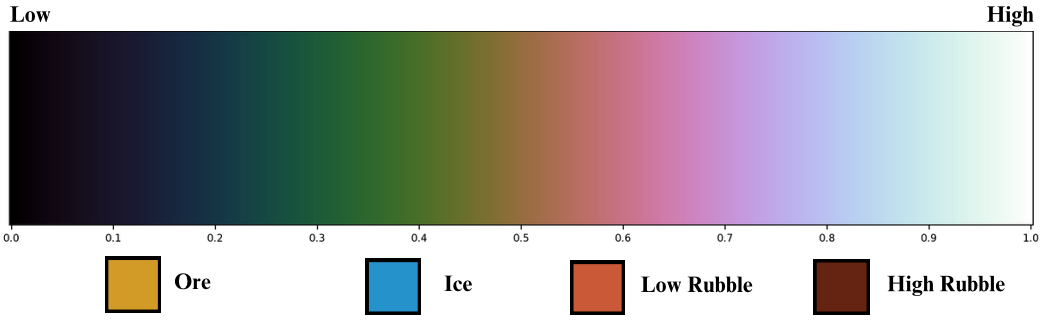
\includegraphics[width=\linewidth]{images/methods_mono/factory_placement/grad.png}
        \captionsetup{justification=justified, singlelinecheck=false, width=1\linewidth, labelfont=bf} 
        \caption{The legend image provided below accompanies subsequent images. It illustrates the original starting map of the Lux environment. The gradient color scheme represents the presence of elements, with lighter colors indicating lower presence and darker colors indicating higher presence. The color mapping for ore, ice, and rubble remains consistent with previous representations (\autoref{fig:lux-map}).}
        \label{fig:grad-image}
    \end{minipage}\hfill
    \centering
    \begin{minipage}{1\textwidth}
        \centering
        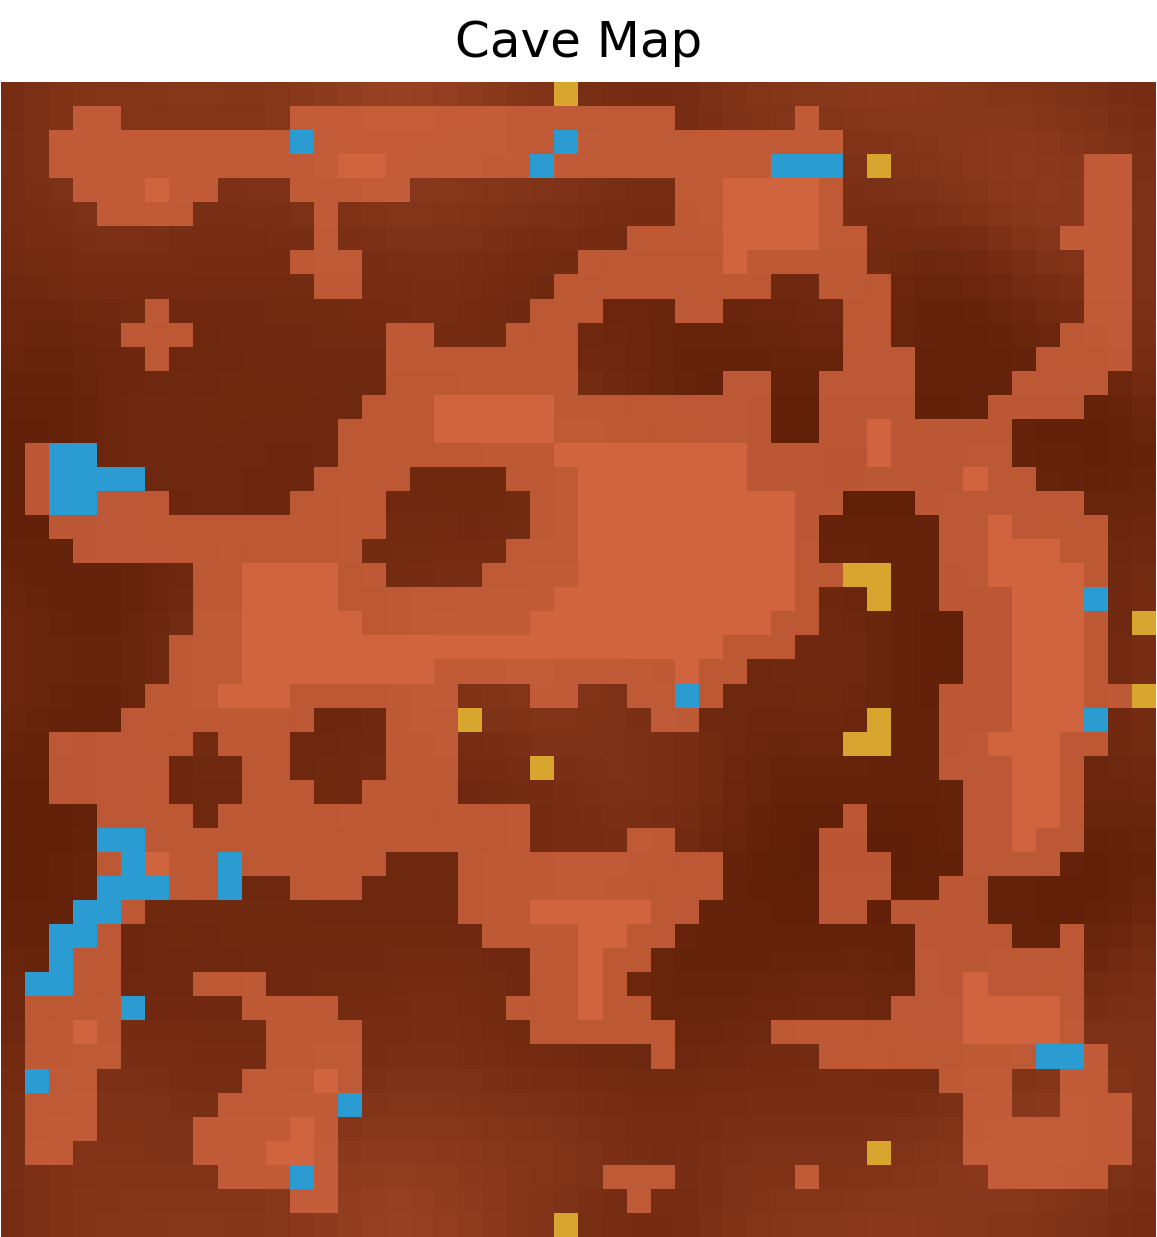
\includegraphics[width=0.38\linewidth]{images/methods_mono/factory_placement/cave_map.png}
        \captionsetup{justification=justified, singlelinecheck=false, width=1\linewidth, labelfont=bf} 
        \caption{Image of the original starting seed of the map without any factories placed on it, generated as the initial step before the bidding phase \protect \footnotemark.}
        \label{fig:grad-map}
    \end{minipage}\hfill
    \vspace{8pt}
    
    \begin{minipage}{0.32\textwidth}
        \centering
        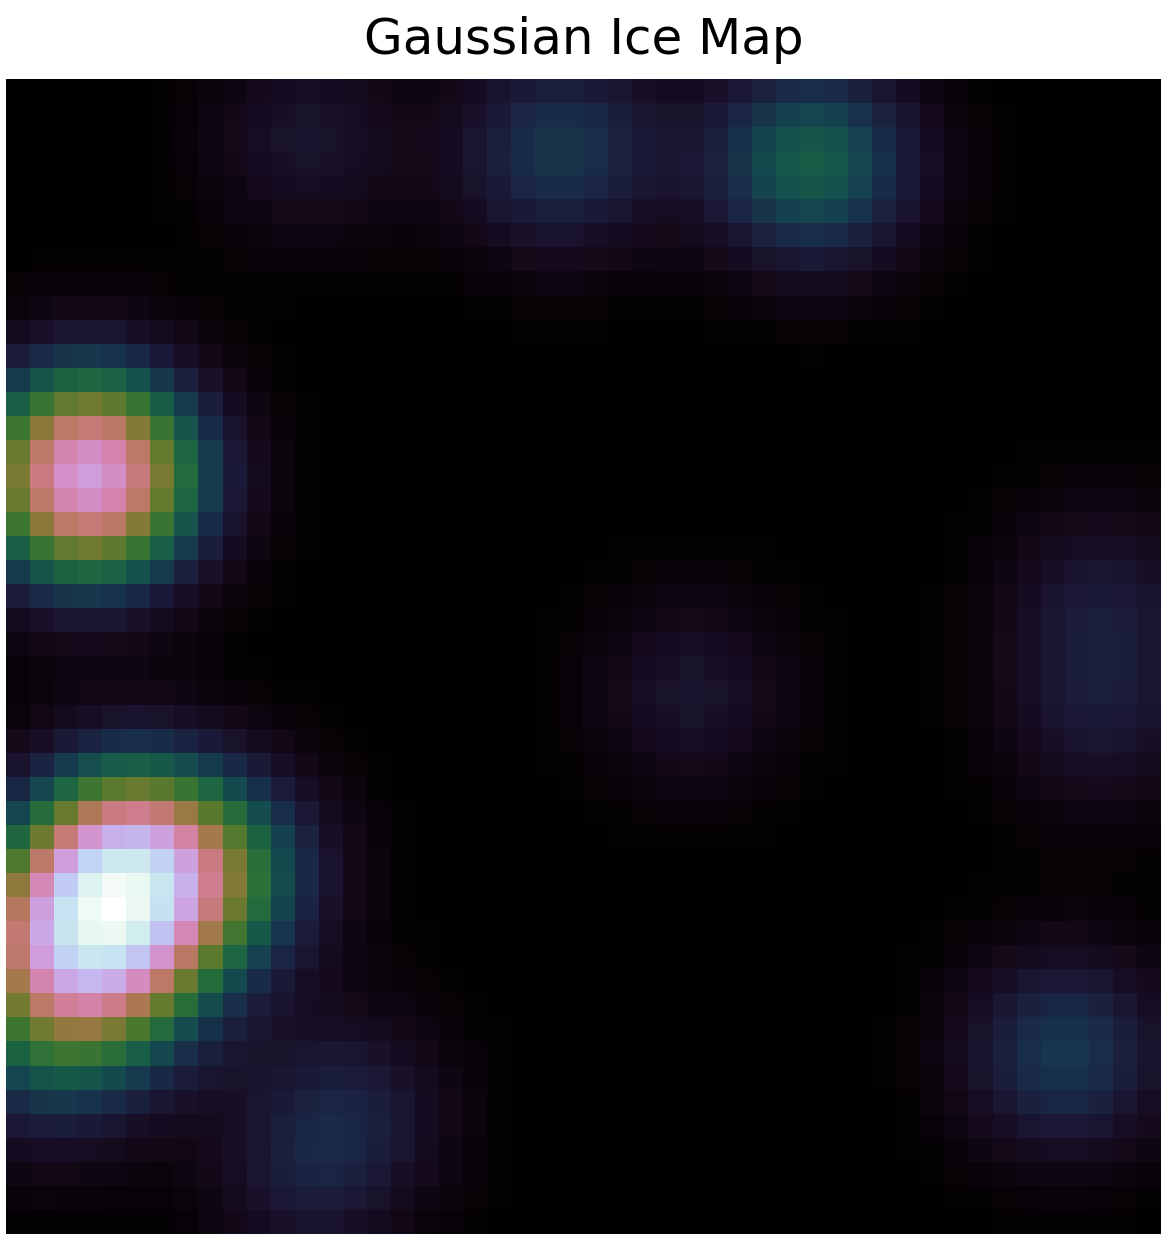
\includegraphics[width=\linewidth]{images/methods_mono/factory_placement/gaussian_ice_map.png}
        \captionsetup{justification=justified, singlelinecheck=false, width=1\linewidth, labelfont=bf} 
        \caption{High presence of ice calculated using our Gaussian filter. Lighter values indicate high-density ice areas.}
        \label{fig:gaussian-ice}
    \end{minipage}\hfill
    \begin{minipage}{0.32\textwidth}
        \centering
        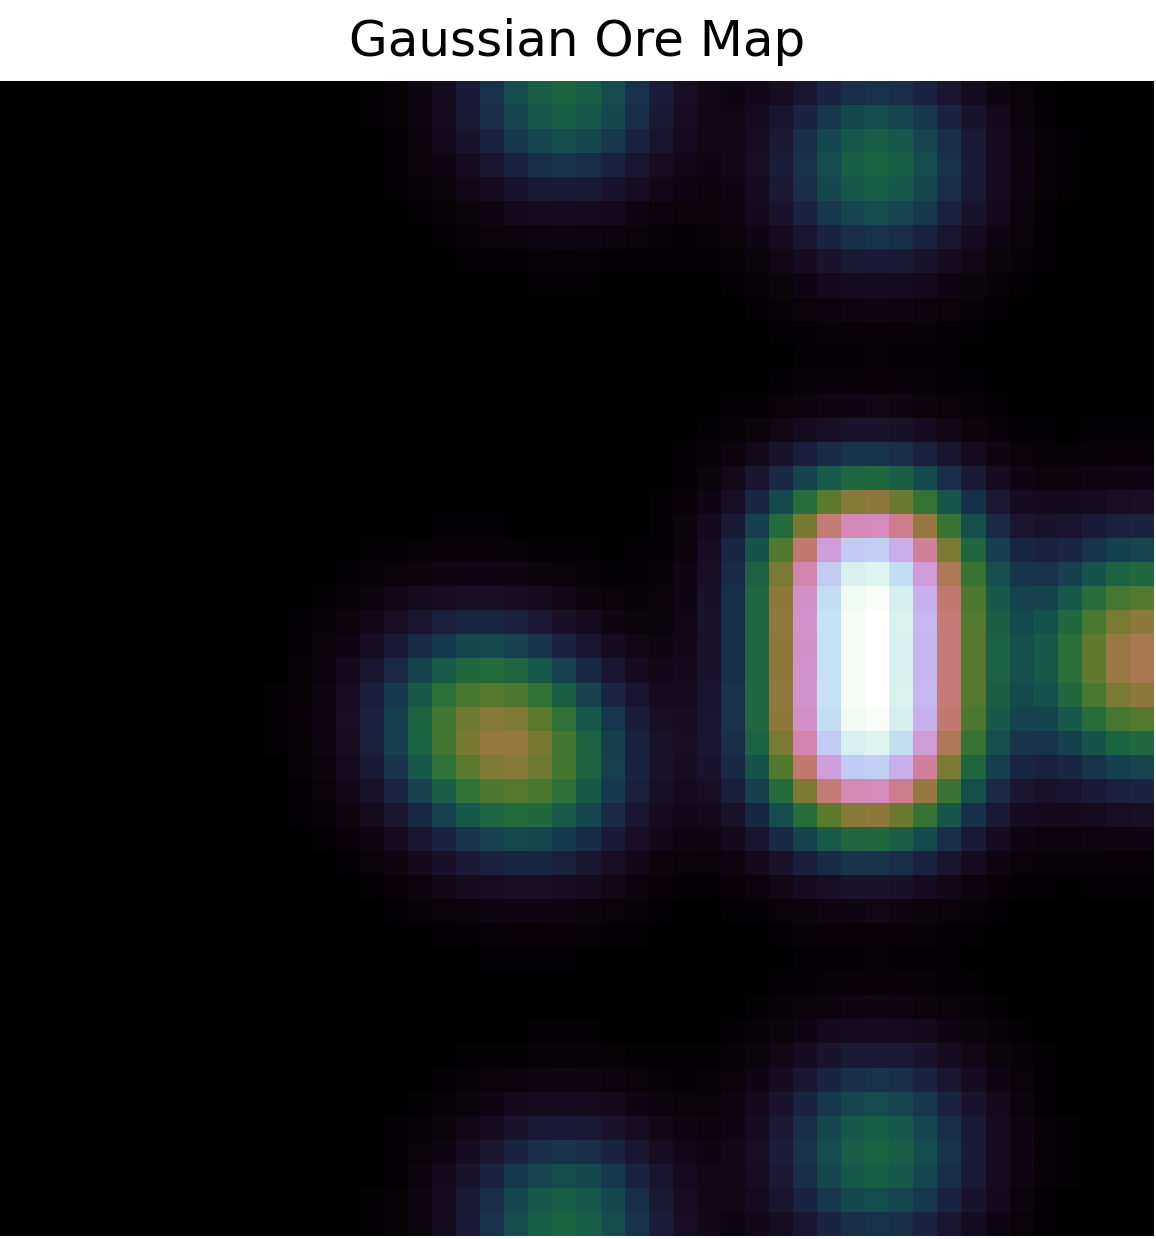
\includegraphics[width=\linewidth]{images/methods_mono/factory_placement/gaussian_ore_map.png}
        \captionsetup{justification=justified, singlelinecheck=false, width=1\linewidth, labelfont=bf} 
        \caption{High presence of ore calculated using our Gaussian filter. Lighter values indicate high-density ore areas.}
        \label{fig:gaussian-ore}
    \end{minipage}\hfill
    \begin{minipage}{0.32\textwidth}
        \centering
        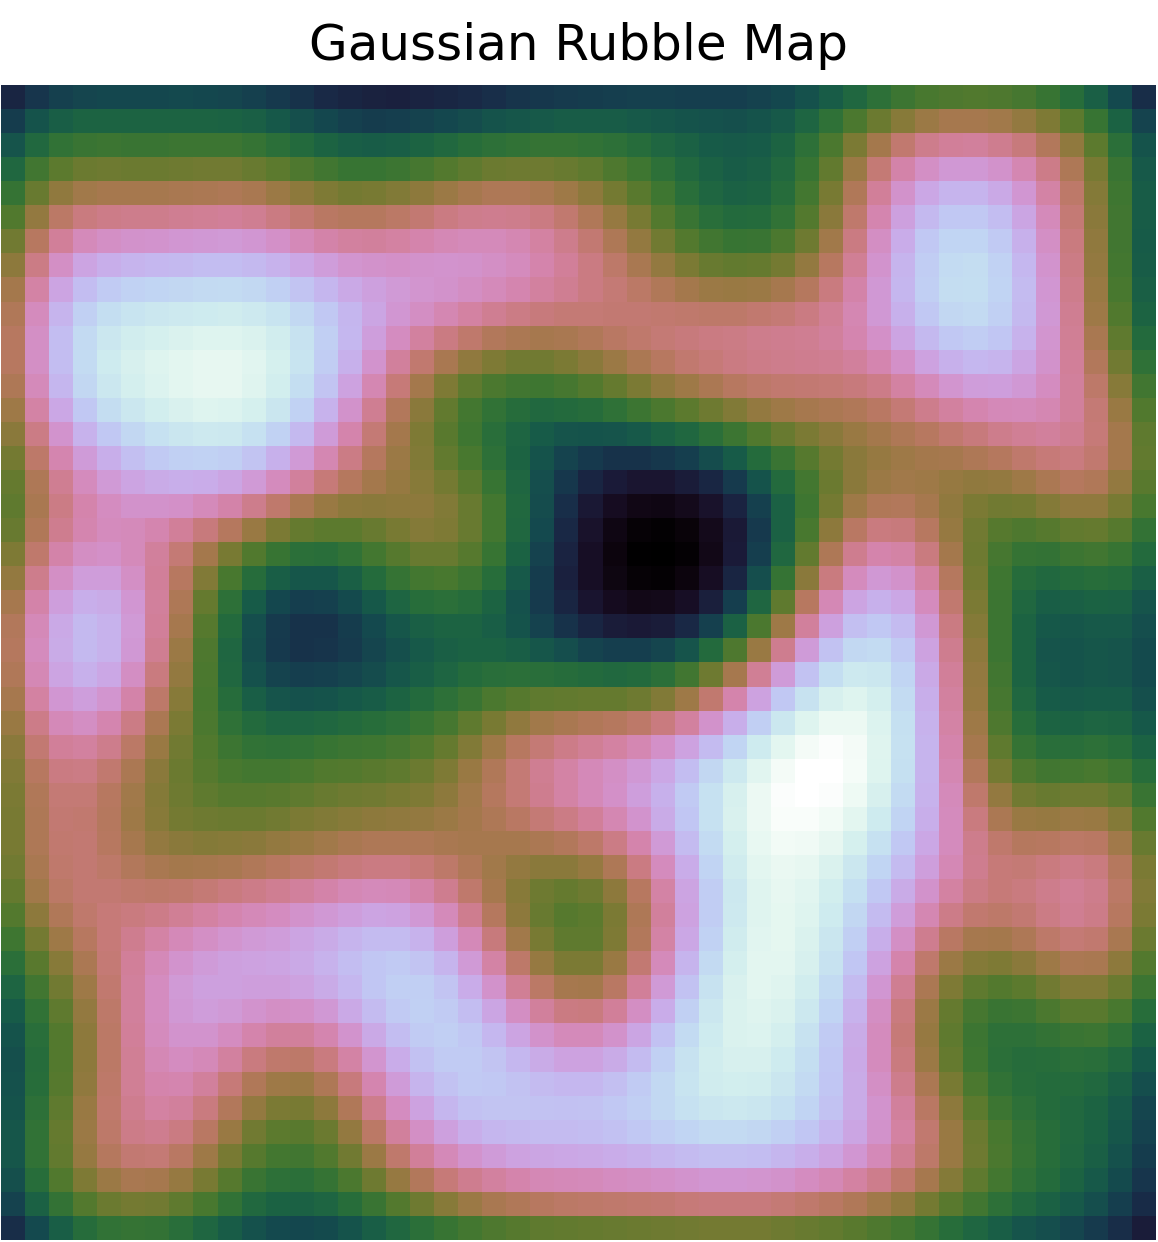
\includegraphics[width=\linewidth]{images/methods_mono/factory_placement/gaussian_rubble_map.png}
        \captionsetup{justification=justified, singlelinecheck=false, width=1\linewidth, labelfont=bf} 
        \caption{High presence of rubble calculated using our Gaussian filter. Lighter values indicate high-density rubble areas.}
        \label{fig:gaussian-rubble}
    \end{minipage}
\end{figure}


\footnotetext{The seed used to generate the cave-style map was set to 420.}


\begin{figure}[htbp]
    \centering
    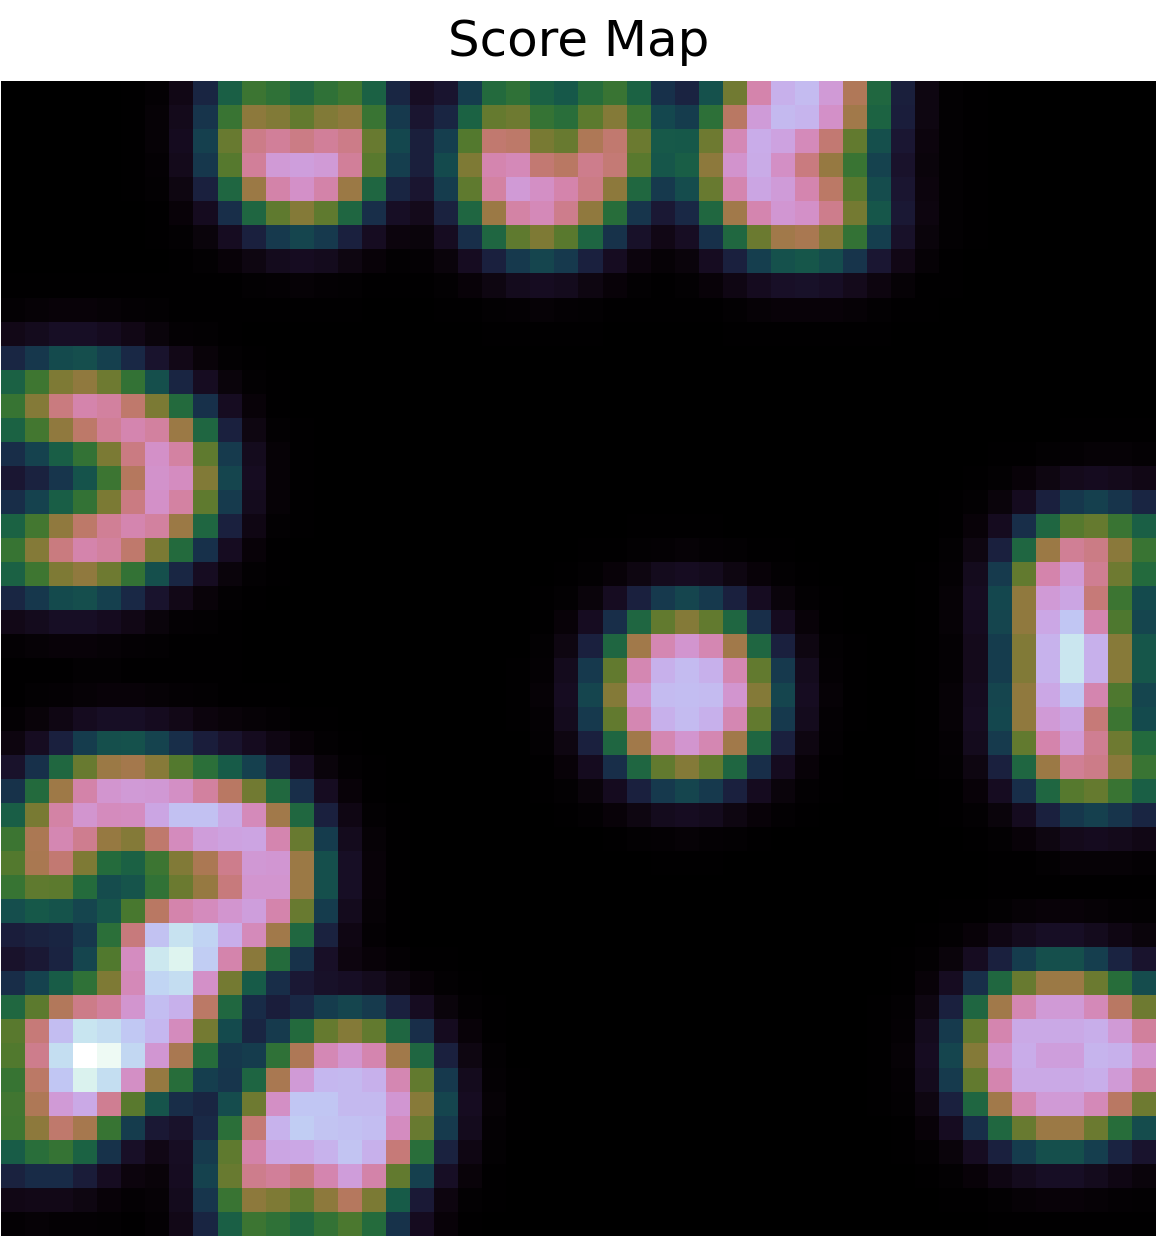
\includegraphics[width=0.5\linewidth]{images/methods_mono/factory_placement/score_map.png}
    \captionsetup{justification=justified, singlelinecheck=false, width=1\linewidth, labelfont=bf} 
    \caption[]{The output of the Gaussian filter algorithm applied to the ore, ice, and rubble maps weighted with possible spawn position maps \protect\footnotemark. Lighter areas indicate the best possible spawn locations.}
    \label{fig:score-map}
\end{figure}

\footnotetext{The possible spawn positions are represented by a mask matrix where True values indicate valid spawn positions and False values indicate invalid ones. Invalid positions for factories include those on top of ore blocks, ice blocks, or the very edges of the map. This information is provided and calculated by the Lux AI engine.}

\subsection{Actions}
\label{subsec:mono-actions}

\noindent Utilizing a single actor, we compressed our action space into a single discrete space, accommodating both unit and factory actions. To ensure precise probability calculations and to restrict factory actions for units, and vice versa, we \textbdd{employed invalid action masks}. This essentially led to a theoretical \textbdd{splitting of the action space} into two categories: factory actions and unit actions. Factory actions were masked out for all units, and unit actions were masked out for all factories, with the exception of the no-operation action, which was available to both entity types. Restricting illegal actions within such vast action spaces is crucial for expedited learning. For instance, by forbidding the transfer action when no cargo is available on the unit or when the unit is not adjacent to another unit, or when the factory is not adjacent to the unit, we effectively reduced the range of possible unit actions from 13 to 8 (including move in 4 cardinal directions, pickup, dig, recharge, and no-operation) (\autoref{subsec:lux-action}). Although we did not implement a more complex masking system to limit repeated actions or prevent agents from overlapping, as it would introduce excessive logic and determinism into the game, we aimed for the central decision maker to \textbdd{learn these patterns} rather than explicitly instructing it on all possible negative edge cases. Lichen watering was also excluded for all factories to better align them with the task of preserving their longevity, as watering lichen consumes water, thereby reducing factory lifespan. For global control, our final action space was of size $[16,48,48]$, where each pixel on the map had an assigned action vector, as illustrated in \autoref{fig:action_space_mono}.

\begin{figure}[htbp]
    \centering
    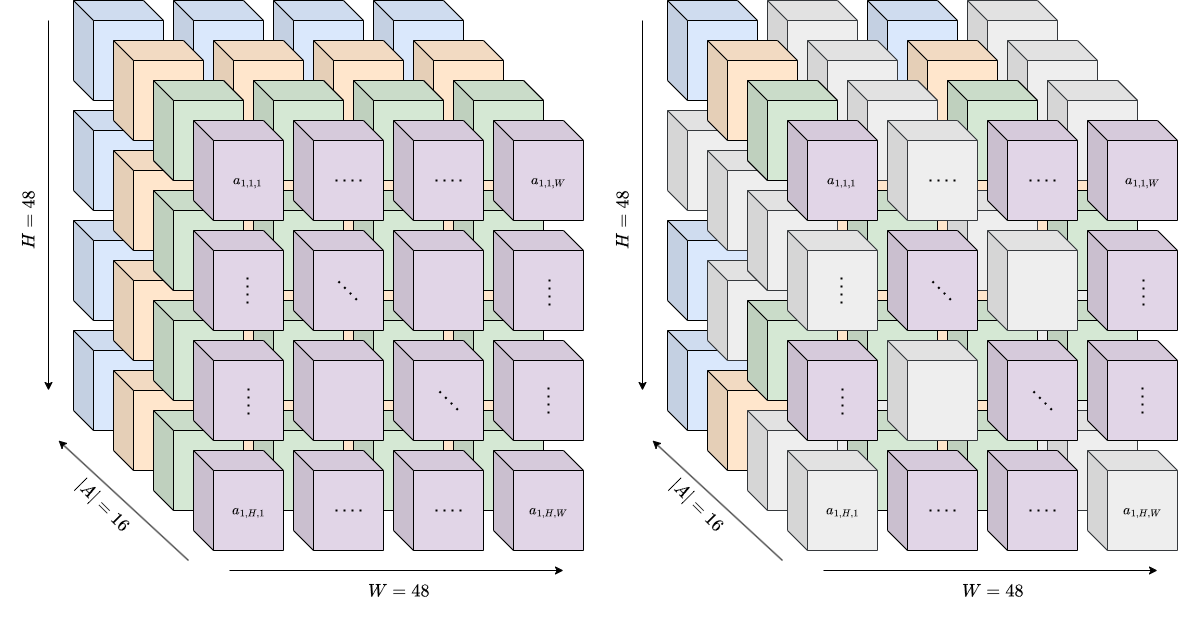
\includegraphics[width=0.5\linewidth]{images/methods_mono/action/action_space.png}
    \captionsetup{justification=justified, singlelinecheck=false, width=1\linewidth, labelfont=bf} 
    \caption[]{A comprehensive representation of an action tensor is depicted on the left, alongside its masked version utilizing invalid action masking. Here, \textbdd{masked out} refers to actions that are deemed invalid in the environment given a state $s$. Similarly, colored boxes indicate the same actions across different pixels of the environment. This representation has limitations, as it shows each pixel on a $4\times4$ grid with $4$ possible actions each. From the illustration, it is also visible that invalid action masking effectively reduces the exploration space of the environment for the learner agent.}
    \label{fig:action_space_mono}
\end{figure}

\subsection{Observation}
\label{subsec:mono-observation}

\noindent The observation features were also overhauled from the single-unit testbench (\autoref{subsec:single-observation}), aiming to create a compact observation space while still providing the model with all relevant information. These features can be categorized into four groups: \textbdd{global features, map features, unit features, and factory features}. Global features consist of scalar values that are tiled to the shape of the map for concatenation with other features. Map, unit, and factory features are all shaped \textbdd{H x W}, where \textbdd{H} represents the game board's height and \textbdd{W} its width, describing the tile of the board, units, and factories respectively. Features are represented as 32-bit floating-point numbers. Boolean flags are converted to zeros and ones, while other values are normalized to a \textbdd{[-1, 1] range} to aid convergence. All features are concatenated as channels into a single tensor within the model. See \autoref{tab:features} for a complete list of features.

\bigskip

\noindent The model additionally receives two matrices, each cell containing the ID of the unit or factory occupying that position on the map, representing the entity's team affiliation. These matrices do not alter entity behavior but are utilized during training for reward assignment, critic values, log probabilities, and entropy values. Further details on reward assignment will be provided in \autoref{subsec:grouping}.

\begin{table}[htbp]
    \centering
    \begin{tabular}{cccc}
        \hline
        Feature Type & Feature Name & Shape & Value Range \\
        \hline
        Global & Step & Scalar & [-1, 1] \\
        Global & Daytime & Scalar & \{0, 1\} \\
        \hline
        Map & Friendly Factory & H x W & \{0, 1\} \\
        Map & Ice & H x W & \{0, 1\} \\
        Map & Ore & H x W & \{0, 1\} \\
        Map & Rubble & H x W & [-1, 1] \\
        Map & Friendly Unit & H x W & \{0, 1\} \\
        Map & Enemy Unit or Factory & H x W & \{0, 1\} \\
        \hline
        Unit & Heavy Unit & H x W & \{0, 1\} \\
        Unit & Power in Battery & H x W & [-1, 1] \\
        Unit & Ice in Cargo & H x W & [-1, 1] \\
        Unit & Ore in Cargo & H x W & [-1, 1] \\
        \hline
        Factory & Power in Factory & H x W & [-1, 1] \\
        Factory & Ice in Factory & H x W & [-1, 1] \\
        Factory & Water in Factory & H x W & [-1, 1] \\
        Factory & Ore in Factory & H x W & [-1, 1] \\
        Factory & Metal in Factory & H x W & [-1, 1] \\
        \hline
    \end{tabular}
    \captionsetup{justification=justified, singlelinecheck=false, width=1\linewidth, labelfont=bf}
    \caption{Table containing the complete list of observation features, along with their shape and value range.}
    \label{tab:features}
\end{table}

\subsection{Residual Network} \label{subsec:residual}

\noindent Residual Networks were developed as a response to the increasing complexity of model depth in image recognition tasks. Progressing from AlexNet (\textcolor{deepblue}{\cite{AlexNet}}) to VGG16 (\textcolor{deepblue}{\cite{simonyan2015deep}}), GoogLeNet (\textcolor{deepblue}{\cite{szegedy2014going}}), and finally to ResNet-50 (\textcolor{deepblue}{\cite{he2015deep}}), which has a depth of 50 layers, ResNets introduced a crucial feature called \textbdd{residual} or \textbdd{skip connections} (\textcolor{deepblue}{\autoref{fig:residual-net}}). These connections allow layers to receive information not only from adjacent layers but also from earlier layers via direct links, creating a parallel path for more effective information flow. Highlighted in the seminal paper by the Microsoft Research team, ResNets, despite their lower complexity relative to VGG-16, achieved an 8x increase in depth with 152 layers and recorded a $3.57\%$ error rate on the ImageNet dataset (\textcolor{deepblue}{\cite{he2015deep}}). This architecture's efficiency comes from its ability to enable later layers to learn only the \textbdd{residual differences} from their inputs rather than the entire function mapping. Specifically, if the desired output $H(x)$ is defined as $H(x)=F(x) + x$, where $F(x)$ represents the residual mapping to be learned, thus the network effectively learning an identity function when $F(x)=0$, i.e., when there is no difference between $x$ and $H(x)$.

\bigskip

\begin{figure}[htbp]
    \centering
    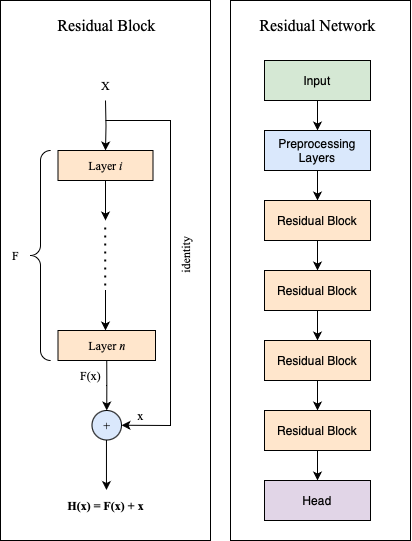
\includegraphics[width=0.45\linewidth]{images/methods_mono/residuals/residual_net.png}
    \captionsetup{justification=justified, singlelinecheck=false, width=1\linewidth, labelfont=bf} 
    \caption[]{A representation of a residual block and its utilization in Residual Networks, which usually include preprocessing layers, which can vary by input type. For images, this often involves convolution layers coupled with max pooling and ReLU activations. The network's head typically consists of a sequence of linear projection layers.}
    \label{fig:residual-net}
\end{figure}


\noindent Residual connections address the challenge posed by extremely deep networks, where during the lengthy backpropagation process, the gradients of the loss functions can diminish to the point of vanishing. This premature vanishing effectively halts the learning process. By implementing residual connections, there is improved gradient flow throughout the network, which not only counters the \textbdd{vanishing gradient problem} but also helps prevent overfitting and deterioration of the model's performance. Residual networks address the gradient vanishing problem by functioning as an ensemble of shallow networks, which helps to avoid the issues associated with gradient explosions rather than directly solving them. This architectural approach is particularly beneficial in reinforcement learning tasks where the environment requires complex representations, enabling deeper networks to learn more effective mappings from inputs to outputs.

\subsection{Leaky ReLU}
\label{subsec:leaky-relu}

\noindent Leaky Rectified Linear Unit (Leaky ReLU) (\cite{xu2015empirical}) is a variant of the popular Rectified Linear Unit (ReLU) (\cite{agarap2019deep}) activation function. While ReLU sets negative values to zero, Leaky ReLU \textbdd{introduces a small, non-zero slope for negative inputs}. Unlike ReLU, the slope coefficient in Leaky ReLU is pre-defined and remains fixed throughout training, rather than being learned. This activation function is particularly useful in scenarios where \textbdd{sparse gradients} are a concern, such as training generative adversarial networks or actor-critic networks in reinforcement learning. In these contexts, maintaining non-zero gradients for negative inputs helps prevent the issue of "dying ReLU" (\cite{Lu_2020}).

\bigskip

\noindent By allowing gradients to propagate even for negative inputs, Leaky ReLU effectively prevents them from vanishing, promoting more stable learning. Moreover, it \textbdd{pairs well with} techniques like \textbdd{orthogonal weight initialization}. It's important to note that the choice of activation function and weight initialization method can significantly impact the training dynamics and performance of neural networks. Therefore, careful consideration of these factors is essential for achieving optimal results in various tasks and domains (\cite{datta2020survey}; \cite{shengyi2022the37implementation}).

\begin{figure}[htbp]
    \centering
    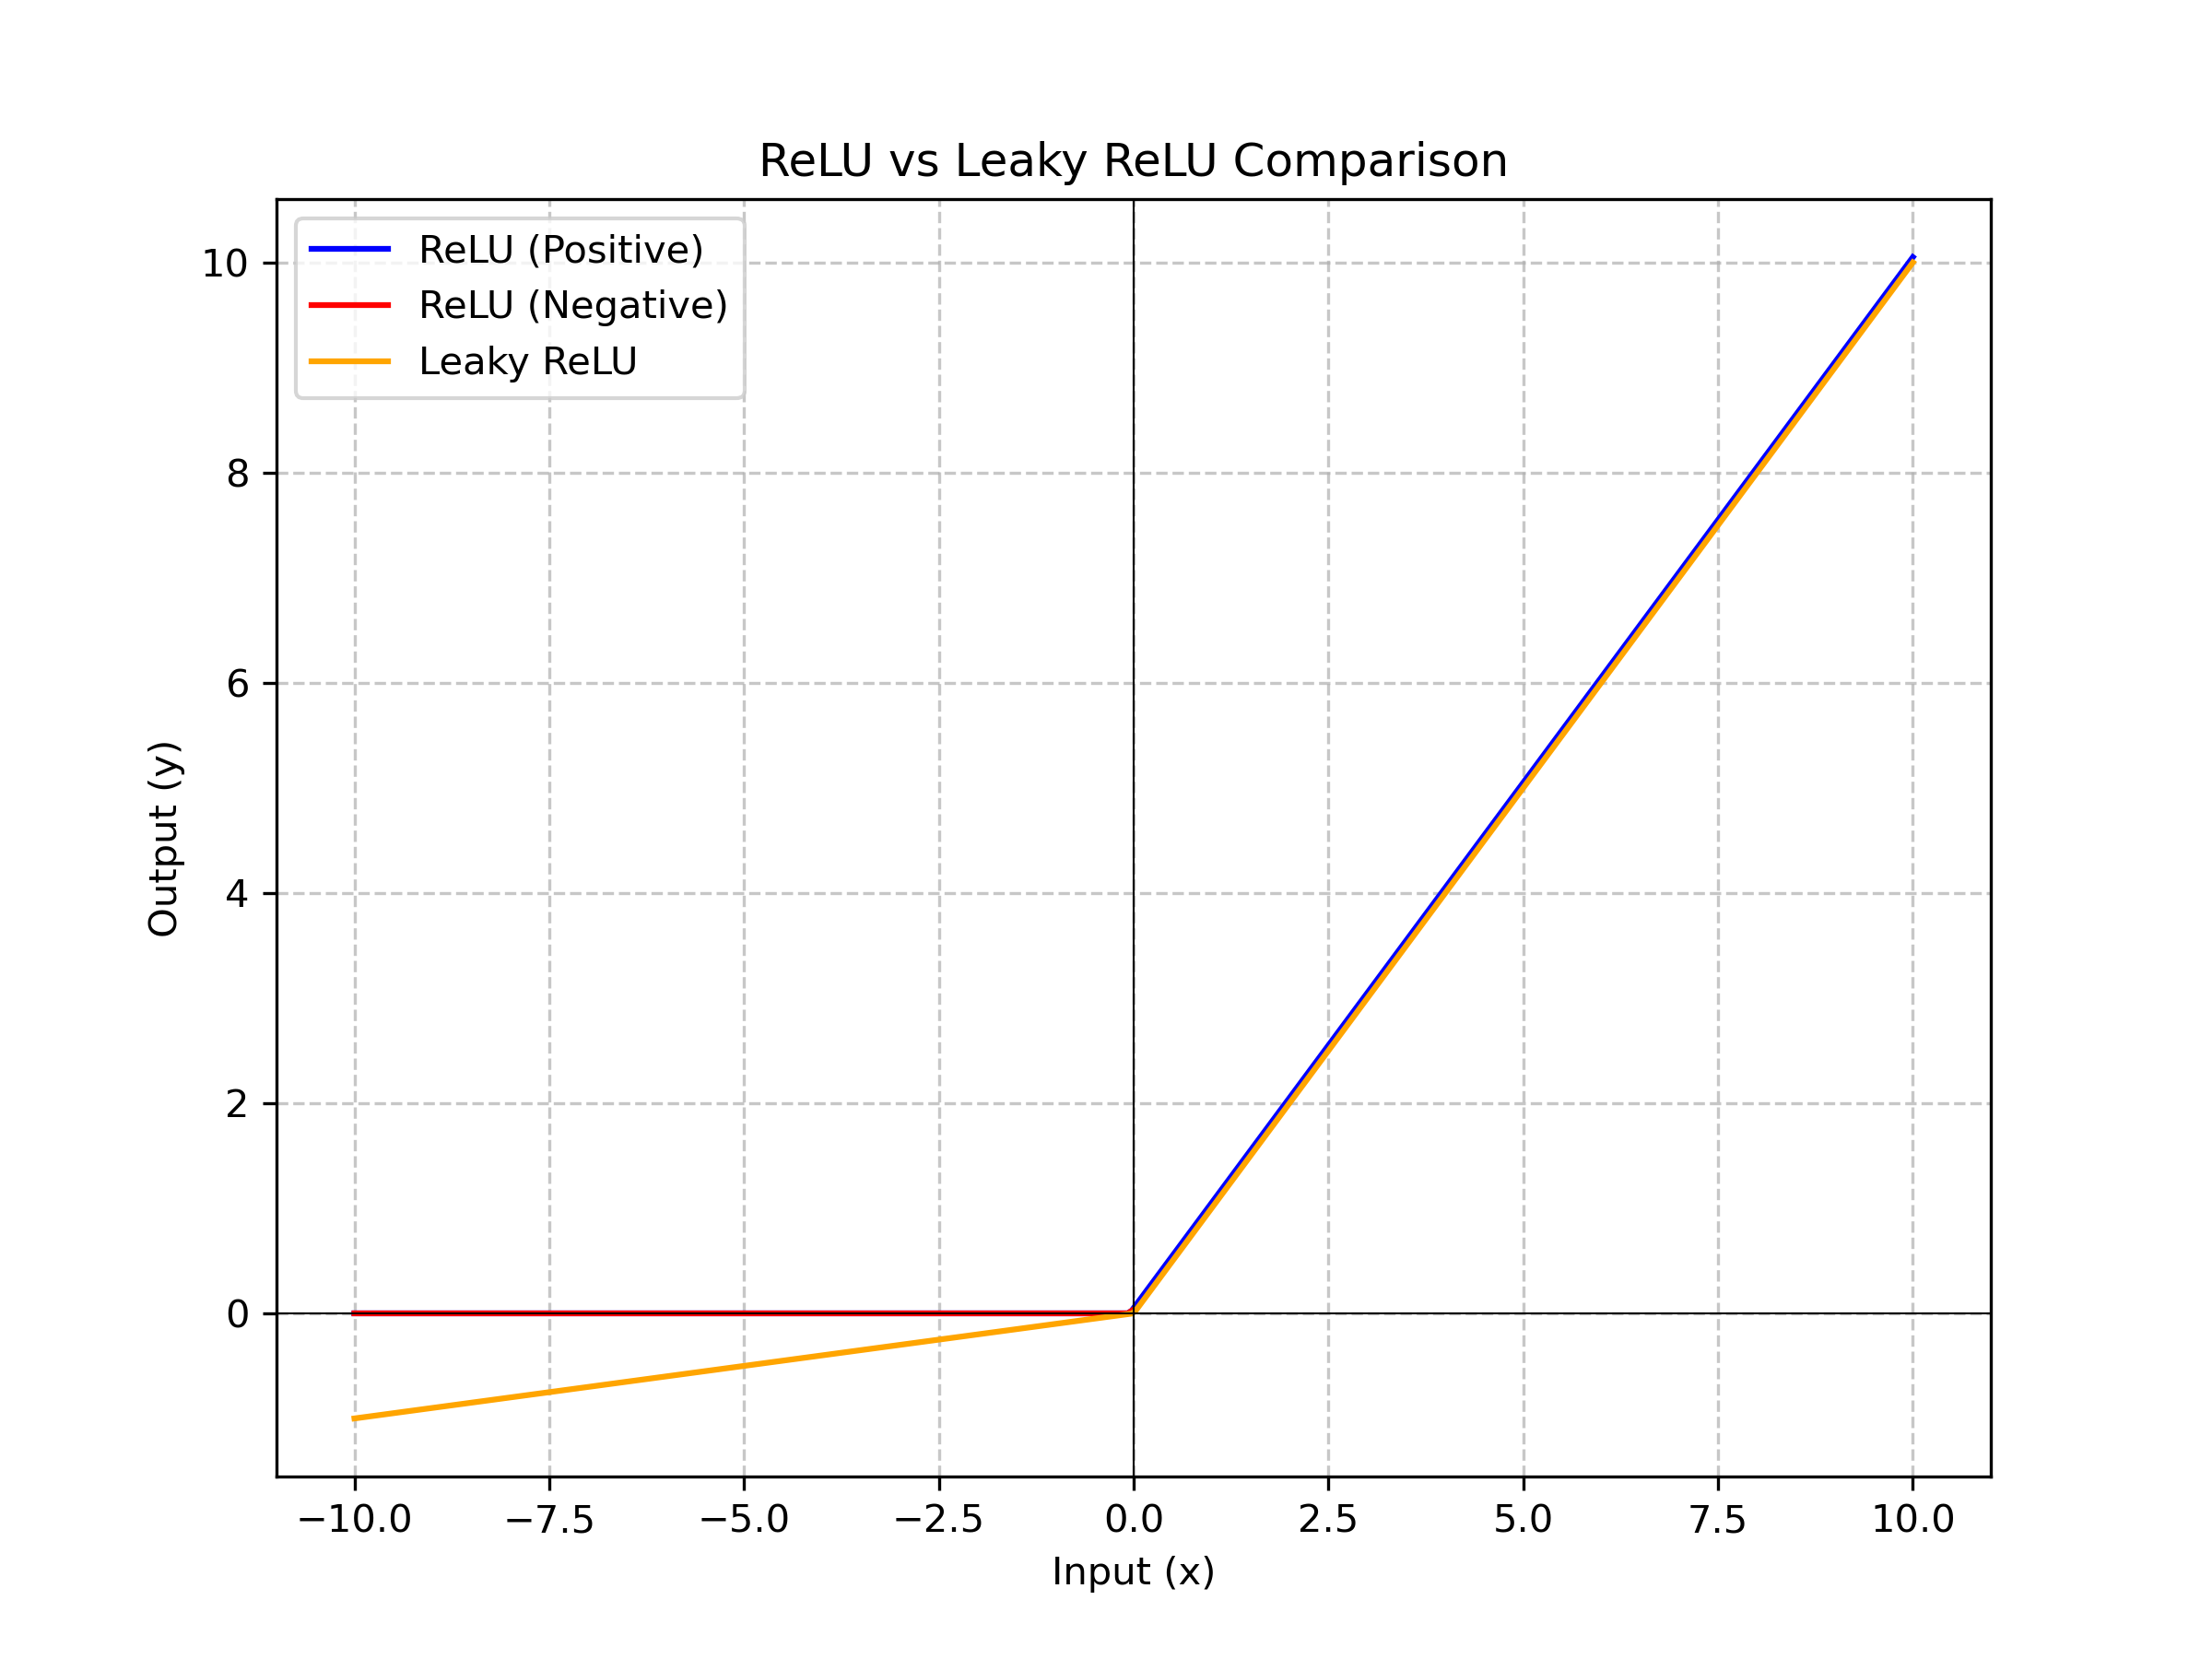
\includegraphics[width=0.7\linewidth]{images/methods_mono/leaky_relu/leaky_relu.png}
    \captionsetup{justification=justified, singlelinecheck=false, width=1\linewidth, labelfont=bf} 
    \caption[]{The figure illustrates the limitation of the popular ReLU activation function, which creates a "dead zone" where negative inputs are squashed to zero. In contrast, Leaky ReLU addresses this issue by allowing negative outputs as well, introducing a small, pre-defined slope for negative inputs. This slope, typically fine-tuned for specific tasks, prevents the dead zone and ensures gradients can flow even for negative inputs. We used the default value for this slope, which is set to 0.01 in the official PyTorch implementation (\cite{pytorchinit}).}
    \label{fig:leaky-relu}
\end{figure}

\subsection{Squeeze-and-Excitation Block} \label{subsec:se}

\noindent The concept behind Squeeze and Excitation networks is straightforward: to enhance the performance of ResNets with minimal computational overhead, thus optimizing the performance tradeoff (\textcolor{deepblue}{\cite{hu2017squeezeandexcitation}}). The approach involves adding parameters to each channel of a convolutional block, allowing the network to adaptively adjust the weighting of each feature map. This enables the network to learn an ordering of \textbdd{feature map importance}, effectively prioritizing certain features. This method is similar to feature selection techniques in machine learning (\textcolor{deepblue}{\cite{FeatureSelection}}), but with the key difference that it is learned dynamically by the network.

\bigskip

\begin{figure}[htbp]
    \centering
    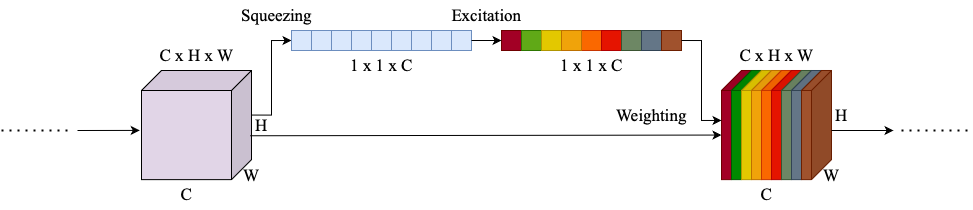
\includegraphics[width=1\linewidth]{images/methods_mono/se_block/se_layer.png}
    \captionsetup{justification=justified, singlelinecheck=false, width=1\linewidth, labelfont=bf} 
    \caption[]{The figure illustrates how the channel-wise aggregation and self-gating mechanism generate per-feature channel weights for the original input. This process highlights the sequential transformation from spatial aggregation to the modulation of feature importance.}
    \label{fig:seop}
\end{figure}

\noindent After the residual layers, the network branches into a \textbdd{squeezing} path that compresses the input from $H\times W\times C$ to $1\times 1\times C$, effectively creating a channel descriptor that aggregates the feature maps across the spatial dimensions $H$ and $W$ (\textcolor{deepblue}{\cite{hu2017squeezeandexcitation}}). This aggregation is followed by an \textbdd{excitation} operation, a self-gating mechanism that generates per-channel modulation weights from input embeddings. These weights are then applied to scale the channels of the original input $H\times W\times C$, which is then passed to subsequent layers for further processing.

\subsection{Batch Normalization} \label{subsec:batchnorm}

\noindent As networks grew deeper, not only was there a need for residual connections, but also for advanced regularization techniques as well (\cite{TIAN2022146}). Batch normalization has come to light as a suitable solution in response to the challenges of deepening neural networks. Deep networks often employ \textbdd{saturating nonlinearities} or activation functions that lead to a phenomenon known as internal \textbdd{covariate shift} (\cite{ioffe2015batch}). This shift refers to the change in the distribution of network activations due to the updating of network parameters during training. When inputs pass through an activation function, they may be pushed to the extreme values of the function’s range, resulting in saturation. Saturation is problematic because it leads to derivatives near zero, especially noticeable in functions like the sigmoid, which squishes values between zero and one. Consequently, the derivatives at the extremes of the sigmoid function approach zero, causing very small updates during backpropagation (\cite{7376778}). This issue becomes more pronounced as network depth increases, eventually reaching a point where the network cannot effectively update its weights based on the loss function.

\begin{figure}[htbp]
  \centering
  \begin{subfigure}{0.49\textwidth}
    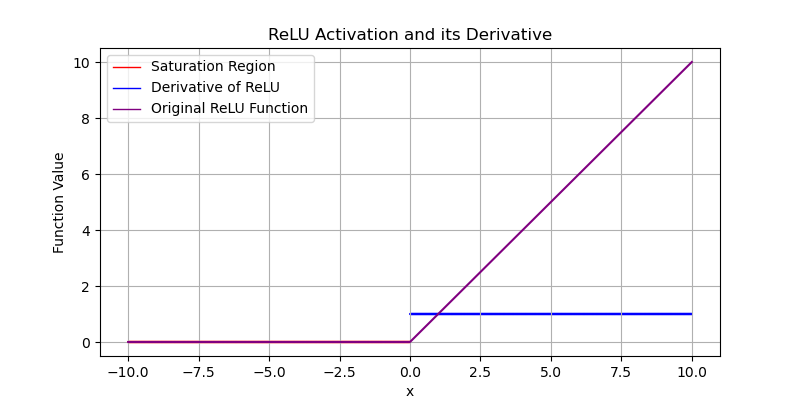
\includegraphics[width=\linewidth]{images/methods_mono/batch_norm/relu.png}
    
    \caption{ReLU nonlinearity.}
    \label{fig:image1}
  \end{subfigure}
  \hfill
  \begin{subfigure}{0.49\textwidth}
    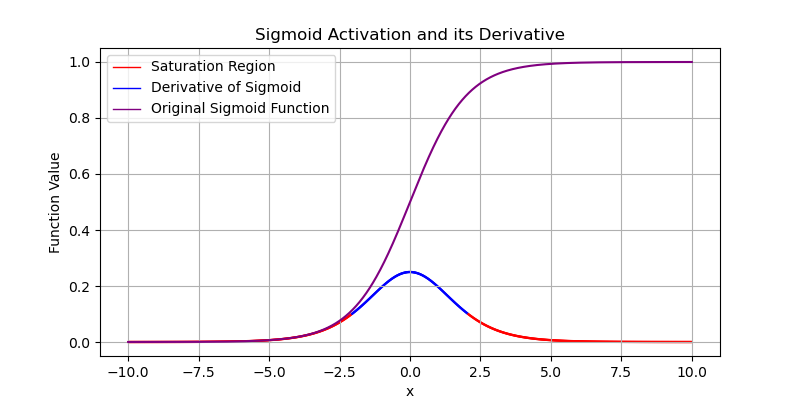
\includegraphics[width=\linewidth]{images/methods_mono/batch_norm/sigmoid.png}
    \caption{Sigmoid nonlinearity.}
    \label{fig:image2}
  \end{subfigure}

  \medskip

  \begin{subfigure}{0.49\textwidth}
    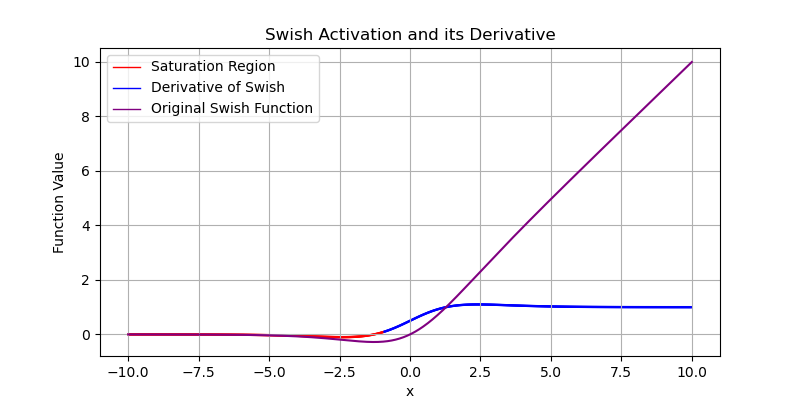
\includegraphics[width=\linewidth]{images/methods_mono/batch_norm/swish.png}
    \caption{Swish nonlinearity.}
    \label{fig:image3}
  \end{subfigure}
  \hfill
  \begin{subfigure}{0.49\textwidth}
    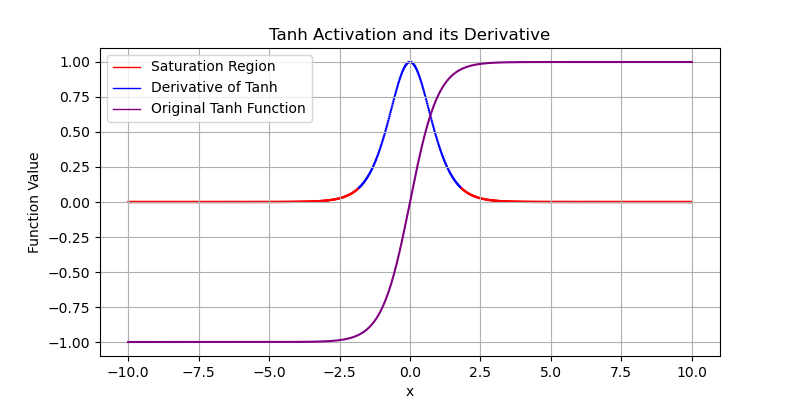
\includegraphics[width=\linewidth]{images/methods_mono/batch_norm/tanh.png}
    \caption{Tanh nonlinearity.}
    \label{fig:image4}
  \end{subfigure}
    \captionsetup{justification=justified, singlelinecheck=false, width=1\linewidth, labelfont=bf} 
  \caption{These figures illustrate various popular activation functions alongside their derivative functions. We highlight regions at the extremes of each function where the derivatives are squished to very small values. In these regions, the network's updates during training are minimal.}
  \label{fig:2x2grid}
\end{figure}

\noindent Batch Normalization originates from the standard practice of normalizing input data to zero mean and unit variance, which optimizes gradient descent by ensuring updates are consistent across all feature dimensions. This uniformity in the loss landscape results in smoother updates. Batch normalization applies this principle to batches of data within the neural network, normalizing the activations from each layer to help the gradients converge more effectively (\cite{ioffe2015batch}).

\bigskip

\noindent Batch normalization utilizes two learnable parameters, beta $(\beta)$ and gamma $(\gamma$), and two non-learnable parameters, the moving averages of mean and variance. The process involves calculating the mean and standard deviation for the batch, normalizing inputs, and then using $\beta$ and $\gamma$ to scale and shift these values. These adjustments allow the activations to shift to means other than zero and variances other than unit variance. The moving averages of mean and variance are updated based on the current batch's calculations. This normalization is performed for each feature channel. By stabilizing the learning process, batch normalization reduces the need for dropout layers, enables \textbdd{higher learning rates}, and decreases dependency on advanced initialization techniques (\cite{ioffe2015batch}).

\bigskip

\noindent In our model, we use batch normalization at \textbdd{each hidden layer}. We decided to apply the normalization \textbdd{before the activation functions} since this is what the original paper's authors suggested. In the layers where batch normalization is enabled, biases are disabled to avoid unnecessary computations (\cite{goodfellow-batchnorm}).

\subsection{Spectral Normalization} \label{subsec:spectralnorm}

\noindent Spectral normalization, originally employed to stabilize the training of \textbdd{discriminator networks} in Generative Adversarial Networks (GANs) (\cite{miyato2018spectral}), has been sparsely adopted for use in actor-critic policy gradient methods in reinforcement learning. In GANs, spectral normalization addresses training instability and the issue of \textbdd{mode collapse}, which occurs when the generated and real distributions become disjoint, leading to vanishing gradients (\cite{yoshida2017spectral}). The structure of GANs, with distinct discriminator and critic networks, is similar to actor-critic methods in reinforcement learning, where actors and critics serve complementary roles. Additionally, Wasserstein GANs (WGANs) utilize the Wasserstein distance (\cite{wiki:Wasserstein_metric}) for their cost function, which provides smoother gradients. However, its effectiveness is based upon adhering to a \textbdd{Lipschitz constraint} $K$. Lipschitz continuous functions restrict how quickly the function values can change, maintaining a slope between any two points that is less than or equal to a constant K, known as the Lipschitz constant (\cite{wiki:Lipschitz_continuity}).

\bigskip

\noindent  This same principle can be applied in actor-critic methods in reinforcement learning, where spectral normalization stabilizes the training of critics by rescaling the weight tensor using the spectral norm $\sigma$, calculated using power iteration methods (\textcolor{deepblue}{\cite{pytorch2}; \autoref{eq:spectral_norm}}). 

\begin{equation}
    W_{\text{sn}} = \frac{W}{\sigma(W)}, \quad \sigma(W) = \underset{h: h \neq 0}{\max}\frac{\left\Vert W h \right\Vert_2}{\left\Vert h \right\Vert_2}
    \label{eq:spectral_norm}
\end{equation}

\noindent When spectral normalization is applied in reinforcement learning, both the actor and critic are trained simultaneously and are interdependent. Applying spectral normalization to the critic helps reduce the risk of \textbdd{policy collapse} (\cite{dohare2023overcoming}), where the actor might learn a suboptimal or \textbdd{degenerate policy}. Furthermore, in policy gradient methods, if learning rates and initialization are not properly managed, one network may dominate the other, leading to an imbalance. Spectral normalization has been demonstrated to increase the generalization and stability of reinforcement learning algorithms, particularly in complex domains such as those involving Atari games, where it has been effectively integrated with Deep Q-Networks (\cite{gogianu2021spectral}).

\subsection{Orthogonal Weight Initialization}
\label{subsec:ortho}

\noindent Weight initialization is essential in deep neural networks as it sets the \textbdd{starting point} for training. Various methods have been employed for this purpose, with random initialization being one of the simplest. In random initialization, weights are assigned values from a normal distribution, which helps mitigate the vanishing gradient problem but can introduce significant variance within the network (\cite{hu2020provable}). Other popular methods include Xavier (\cite{kumar2017weight}) and Kaiming initialization (\cite{he2015delving}), which are effective for shallow and moderately deep networks. For more complex architectures, especially in deeper or recurrent neural networks (RNNs), orthogonal initialization is often used. This technique involves initializing the weights with an \textbdd{orthogonal matrix} (\cite{wiki:Orthogonal_matrix}), a square matrix whose columns and rows are orthogonal unit vectors. This ensures that the weights are independent and maintain equal magnitude.

\bigskip

\noindent Orthogonal initialization offers several benefits, particularly for deep linear networks where it has been shown that the network width necessary for convergence to the global optimum does not depend on depth, unlike other initialization techniques that scale linearly with the number of layers (\cite{hu2020provable}). Additionally, the benefits of orthogonal initialization persist throughout training. This technique is also applied in practical scenarios, for instance, in the implementation of Proximal Policy Optimization (PPO), where it is used to initialize the hidden layers in Mujoco tasks, scaled by $\sqrt{2}$ with biases set to zero (\cite{shengyi2022the37implementation}).

\bigskip

\noindent The scaling factor of the initialization can have a substantial effect on the variance of both the activations and the gradients (\cite{pmlr-v9-glorot10a}). Proper weight initialization for the Rectified Linear Unit (ReLU) activation function with the scale of $\sqrt{2/n_t}$, where $n_t$ is the number of input units to the layer, has been shown to ensure zero mean and unit variance of the outputs (\cite{DBLP:journals/corr/HeZR015}), stabilizing the learning process. Omitting the $n_t$ terms causes higher variance but has been widely used in practice, for which the original PPO implementation is a good example. Since we use Leaky ReLU activations, we used the slightly modified scaling of \autoref{eq:gain}, which was the scaling recommendation for that specific activation in Pytorch (\cite{pytorchinit}).

\begin{equation}
    \text{gain} = \sqrt{\frac{2}{1+\text{negative\_slope}^2}}
\label{eq:gain}
\end{equation}

\bigskip

\noindent Following the recommendations of \cite{shengyi2022the37implementation}, we used the activation function's recommended gain value as the scale for weight initialization in our hidden layers and a scale of 0.01 for the initialization of the actor heads. We initialized the critics with the same scale to get predictions close to zero, matching our scaled-down rewards (\autoref{subsec:hyb-rew}). After learning how much downscaling the weights can help, in some benchmark tests boosting performance by 66\% (\cite{andrychowicz2020matters}), we further scaled down the output layers of the network by a factor of 100 to make the action distribution more closely resemble a uniform distribution. We were still noticing fluctuations in performance based purely on the seed the networks were initialized with, so we performed the same scaling on the critic value output layers' weights and, eventually, the hidden layers.

\subsection{Feature Extractor Model}
\label{sec:monolithic-network}

\noindent We transitioned from a heavily shaped feature space to a \textbdd{CNN-based feature extractor}, aiming to map the observations detailed in section (\autoref{subsec:single-observation}) to an action tensor of size $[16, 48, 48]$. In this representation, 16 signifies the size of the discrete action space, while 48 denotes the map size. Given that both our observation tensor and action space possessed a channel size of 16, encompassing various map, unit, factory, and global features (\autoref{tab:features}), we required a mapping strategy to align the observation space with the action space structure (\autoref{sec:monolithic-network}). We implemented two distinct feature extractor architectures to achieve this goal.

\bigskip

\noindent The first network architecture adopted a U-Net style encoder (\cite{ronneberger2015unet}) with various variations of bottlenecks and a decoder with skip connections (\cite{wu2020skip}). U-Net architectures are well-known for their effectiveness in image segmentation tasks (\cite{ehab2023performance}; \cite{ronneberger2015unet}), and we aimed to achieve a similar outcome but at the \textbdd{entity level segmentation}. Our goal was for the network to recognize that entity-free spaces represented inactive segments of the input space, while units and factories remained segmented as distinct entities. Each entity's class corresponded to the action it performed in the environment. In simpler terms, we aimed to create a segmentation map that \textbdd{established a class system} for each agent, categorizing them into different classes. For instance, if the network predicted a dig action for a unit at a given pixel, it meant that the network had segmented it into a \textbdd{"digger"} class. Similarly, when the model predicted a recharge action, the corresponding agent was categorized into a \textbdd{"recharger"} class within the grid environment.

\bigskip

\noindent The encoder of the network employed \textbdd{Downsampling blocks}, transforming the input tensor from a shape of $[16, 48, 48]$ to $[256,3,3]$. Each Downsampling block comprised a residual block (\autoref{subsec:residual}) and a downsampling convolutional layer with a kernel size of 3 and a stride of 2, effectively \textbdd{halving} the height and width of its input. The residual blocks consisted of 2 convolutional layers, a squeeze-and-excitation layer (\autoref{subsec:se}), and a leaky ReLU (\autoref{subsec:leaky-relu}) as the residual, which was concatenated to the input of the residual block. Spectral (\autoref{subsec:spectralnorm}) and batch normalization (\autoref{subsec:batchnorm}) techniques were applied after each convolutional layer, followed by a leaky ReLU activation function.

\bigskip

\noindent Furthermore, each convolutional layer was initialized using orthogonal initialization techniques (\autoref{subsec:ortho}) based on weighting and gain, following recommendations from the literature (\cite{shengyi2022the37implementation}). To ensure reproducibility and \textbdd{reduce variation in different trial runs}, each layer was hashed and seeded. The Squeeze-and-Excitation module employed a reduction factor of 16, facilitating the calculation of channel weighting and importance for every input channel of the observation feature.

\bigskip

\noindent We explored various bottleneck architectures, including a \textbdd{simple convolutional bottleneck} comprising two residual blocks; a \textbdd{dilated bottleneck} with two 3x3 convolutions with dilation rates of 2 and 4 respectively (\cite{li2018detnet}), followed by a residual block; and a \textbdd{multi-scale bottleneck} incorporating 1x1, 3x3, 5x5, and 7x7 convolution operations to expand the receptive field of the model (\cite{Gao_2021}). The multi-scale U-net architecture, in particular, aims to mitigate degradation issues in target regions of segmentation masks by creating representations of the input on different receptive fields and concatenating them to form a comprehensive feature space representation. This approach has been demonstrated to be effective in maintaining the integrity of target regions in segmentation tasks (\cite{article_bot}; \cite{zhu2024efficient}; \cite{bhojanapalli2020lowrank}). 

\bigskip

\noindent In the decoder component of the network, we designed upsampling blocks that mirrored the structure of the downsampling blocks but in reverse. Each upsampling block begins with a \textbdd{transpose convolution} (\cite{shelhamer2016fully}) to upsample the input feature map, followed by batch and spectral normalization and a leaky ReLU nonlinearity. The block concludes with a residual block, maintaining consistency with the previous structure. The inputs to the upsampling blocks consist of outputs from preceding layers and corresponding residuals from their paired downsampling blocks. We termed this feature extractor network the \textbdd{BottleNet} (\autoref{fig:BottleNet}).

\begin{figure}[htbp]
    \centering
    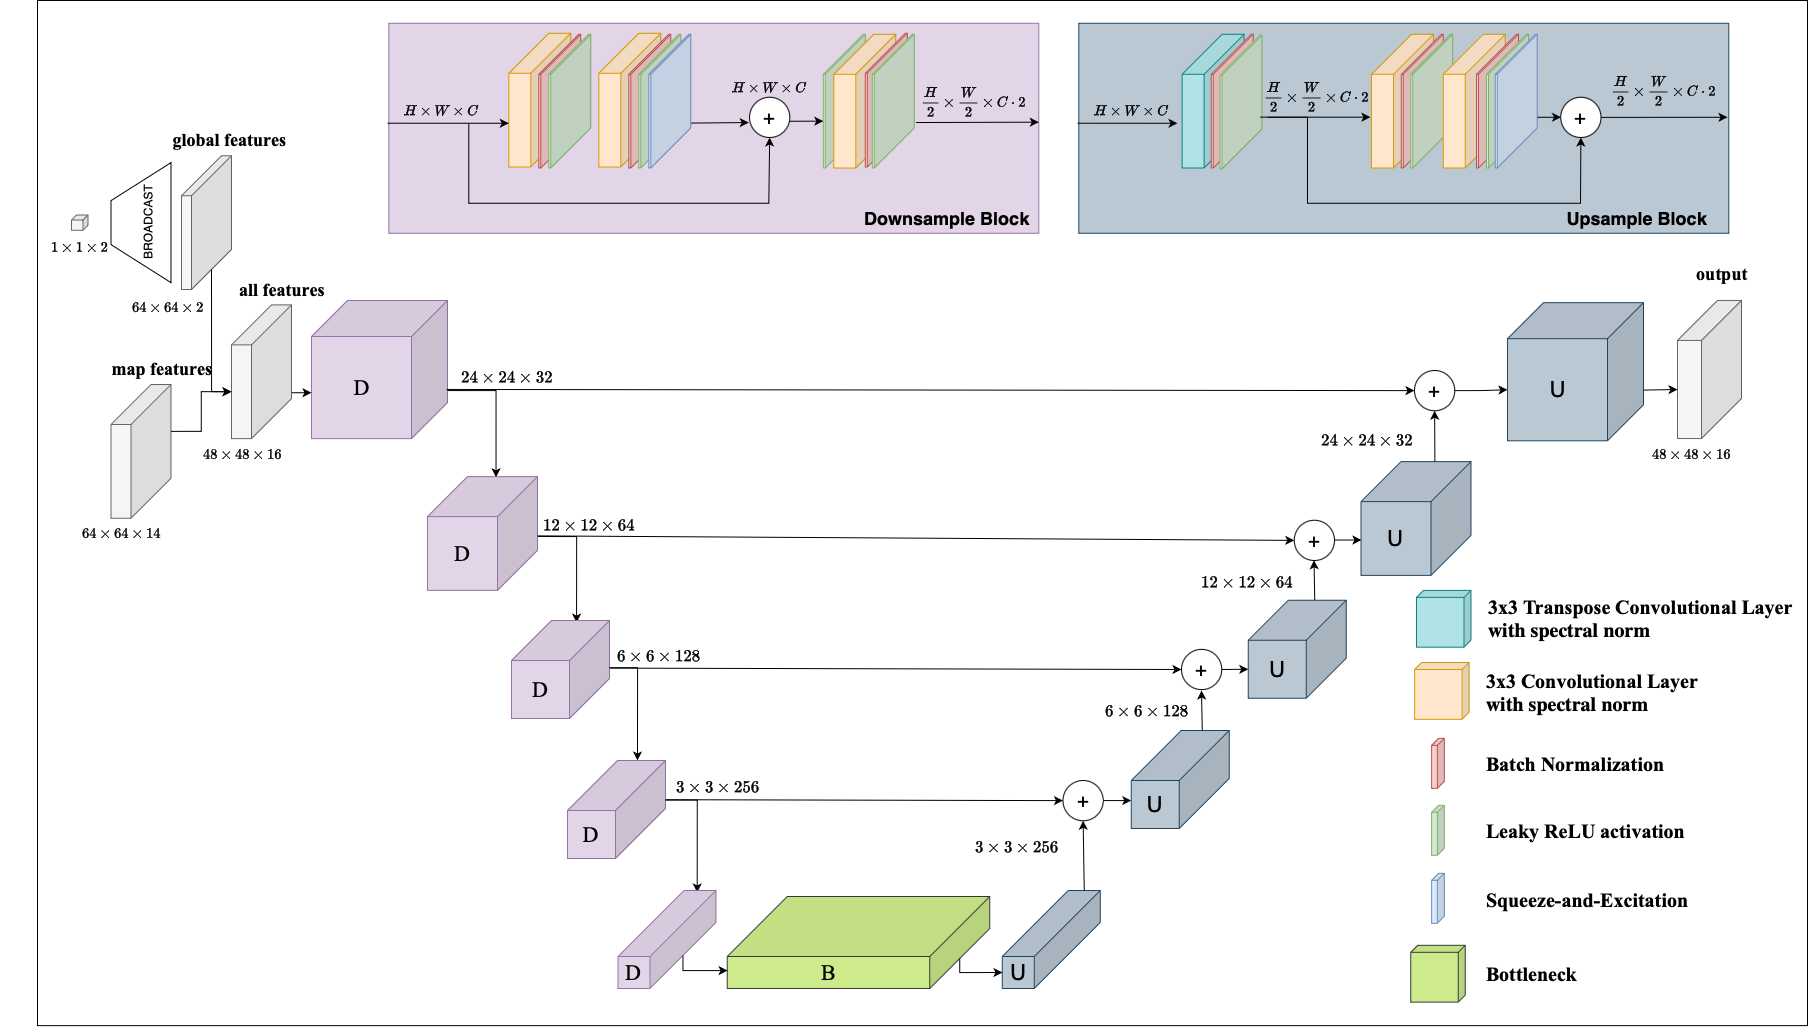
\includegraphics[width=1\linewidth]{images/methods_mono/feature_extractor/unet.png}
    \captionsetup{justification=justified, singlelinecheck=false, width=1\linewidth, labelfont=bf} 
    \caption[]{The figure depicts the entire feature extractor network, encompassing the process from input to output. Map features are combined with tiled-up global features, passing through a sequence of Downsample Blocks until reaching the bottleneck layer. The bottleneck layer's outputs are then upsampled via a series of Upsample Blocks, utilizing matching residuals from downsampling blocks to retain information. Finally, the output is directed towards both the critic and actor networks.}
    \label{fig:BottleNet}
\end{figure}

\begin{figure}[htbp]
    \centering
    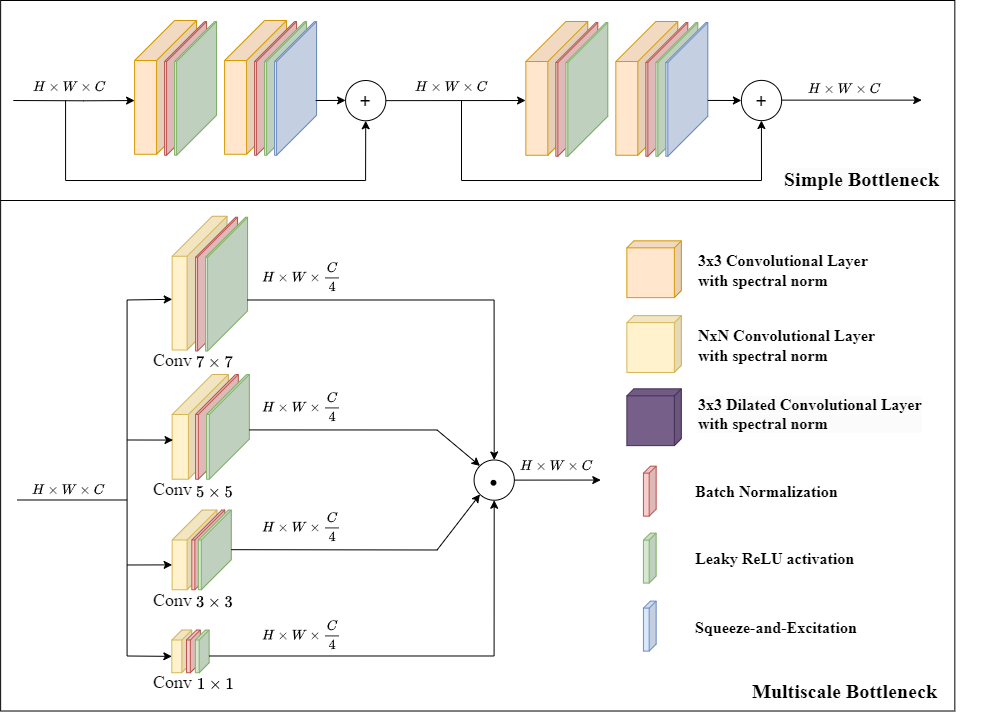
\includegraphics[width=0.9\linewidth]{images/methods_mono/bottleneck/bottleneck.png}
    \captionsetup{justification=justified, singlelinecheck=false, width=1\linewidth, labelfont=bf} 
    \caption[]{The three images illustrate various types of bottlenecks tested for our feature extractor. Starting from the top, the Simple Bottleneck consists of two residual blocks. The Dilated Bottleneck employs convolutional layers with dilation, where the filter expands by a certain factor, allowing it to capture a broader context. Lastly, the Multiscale Bottleneck features a four-branch network, emphasizing important features at different scales.}
    \label{fig:Bottlenecks}
\end{figure}


\noindent For our second network architecture, we opted to maintain the input and output sizes \textbdd{without downscaling}, thus eliminating bottleneck layers. With the goal of creating a one-to-one mapping, we designed a compact residual network that preserves the height and width of the feature maps throughout the network. This network comprises an input convolutional block with spectral normalization, batch normalization, and leaky ReLU nonlinearity. It is followed by four residual blocks, each incorporating SE layers for channel importance weighting, similar to the BottleNet architecture. The final block of this feature extractor network consists of another convolutional block with spectral normalization, batch normalization, and a leaky ReLU activation function. We named this feature extractor the \textbdd{DashNet}.

\subsection{Actor and Critic}
\label{sec:mono-network-actor-critic}

\noindent To ensure compatibility with Stable Baselines, we introduced an additional layer of feature extractor, separated for both the actor and policy networks. To simplify and reduce computational complexity, we passed the output of our feature extractor network through an Identity layer for the actor. Then, for each pixel, its corresponding output value was sent through a linear projection layer, which mapped the extractor network outputs to action \textbdd{loglogits}. For the value network, to fully represent the value of the entire state from the output tensor, we used a single convolutional block paired with layer normalization and leaky ReLU nonlinearity. To refine the representation of value estimates, this mapping compressed the values into a more suitable space, enabling the inclusion of small negative values for more accurate estimates. Next, we employed a \textbdd{global average pooling method} \cite{lin2014network} to average the values of all pixels channel-wise, resulting in a 48x48-sized tensor. This tensor was then flattened and passed through a linear projection layer to produce the final value estimate (\autoref{fig:mono-actor-critic}).

\begin{figure}[htbp]
    \centering
    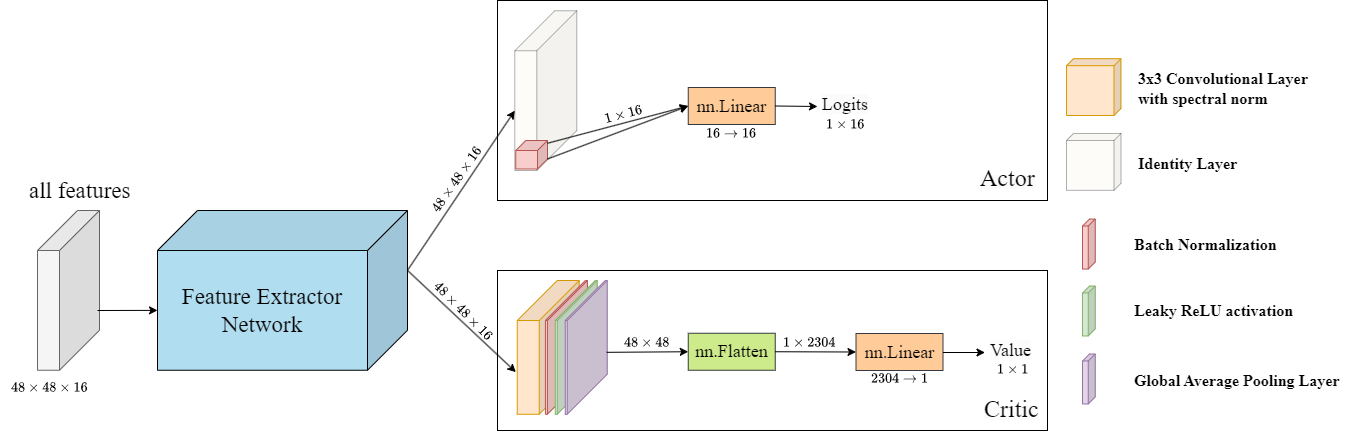
\includegraphics[width=1\linewidth]{images/methods_mono/actor_critic/actor-critic-head.png}
    \captionsetup{justification=justified, singlelinecheck=false, width=1\linewidth, labelfont=bf} 
    \caption[]{The diagram shows the actor and critic heads of the architecture. The actor head extracts action vectors for each pixel using an identity layer and a linear projection for logits. Meanwhile, the value head utilizes a final convolutional block with Global Average Pooling to calculate channel-wise averages, followed by a many-to-one linear projection.}
    \label{fig:mono-actor-critic}
\end{figure}

\subsection{Reward Function}
\label{sec:monolithic-reward-function}

\noindent We adjusted the rewards to incentivize global \textbdd{ice collection, ice transfer, and water generation} in the environment. Ice collection was scaled down by a factor of four to normalize its value to that of water (as 4 ice can be turned into 1 water by the factory). Additionally, we further downscaled the ice collection by a tenth to incentivize not only the digging of ice but also its transfer to factories, which was rewarded 10 times more than simple collection. Water production was rewarded by a single unit, as it is the key metric for sustaining the factory and aligning our model with the task of maintaining factory viability. In order to incentivize units to fill the factories with ice as early as possible, the rewards are \textbdd{multiplied by a factor}, made the following function:

\begin{equation}
    f(\texttt{step}) = 1 + (1000 - \texttt{step}) / 1000 \times 0.1
    \label{eq:reward-early-scaling}
\end{equation}

\noindent This factor \textbdd{boosts the rewards} more the closer we are to the \textbdd{start of the episode}. Our final reward function is the following: 

\begin{align}
    r(\texttt{step}) = \frac{0.01}{f(\texttt{step})} \left[ 
    \frac{\Delta ice\_dug}{40} 
    + \frac{\Delta ice\_transferred}{4} 
    + \Delta water\_produced
    \right]
    \label{eq:reward-mono}
\end{align}

\subsection{Training}
\label{sec:monolithic-approach-training}

\noindent We maintained the training environment and learning algorithm consistent with the single-agent testbench (\autoref{sec:single-unit-testbench}), employing Stable Baselines and its maskable PPO variant (\autoref{subsec:M-PPO}). While Stable Baselines is known for its compatibility with various single-agent environments (\cite{stable-baselines3}), it required significant adaptation for environments where a central decision maker governs actions for multiple entities. Consequently, we underwent a \textbdd{complete rewrite of the PPO learning algorithm} from Stable Baselines to align with our requirements.

\bigskip

\noindent Our action space underwent a transformation from a single discrete 1x12 tensor to a \textbdd{multidiscrete} 16x48x48 tensor. Within each HxW dimension, a 16-dimensional log logit tensor was generated. After exponentiation, an action mask was created for all logits in all HxW dimensions, effectively reducing the corresponding masked values to extremely small numbers, resulting in near-zero probabilities during normalization. Consequently, we had to permute and correctly reshape the action mask and policy head values to tensors of shape 48x48x16. Subsequently, for the calculation of log probabilities, advantages, entropy, and actions, a 48x48 tensor had to be supplied. While further refinements and adjustments were made, detailed discussions on these intricate aspects are omitted here, as they are available in our publicly accessible repository (\url{https://github.com/MagmaMultiAgent}).

\bigskip

\noindent It's crucial to note that implementing self-play in a multi-entity environment using stable baselines is not straightforward (\cite{stable-baselines-issue181}). As a workaround, we employed a passive enemy agent that doesn't interact with the environment. Consequently, our M-PPO algorithm could only learn from the experiences collected by one player, effectively halving the available training data. To compensate for this reduction, we \textbdd{doubled the size of the rollouts} from 4096 to 8192. Additionally, to maintain the desired number of updates during batched gradient descent at 8, we set the minibatch size to 1024. For a comprehensive overview of the hyperparameters and environment settings, please refer to \autoref{app:b}. 

\bigskip

\noindent We originally chose to train the agent over 100k steps, corresponding to 25 evaluation phases, with each phase covering rollouts of size 4096 steps. However, since self-play was not implemented in Stable Baselines (\cite{stable-baselines-issue181}), we extended the training to 200k steps ($8096 \times 25$) to compensate. This ensured that we \textbdd{maintained the same number of model updates} (25), approximating a self-play environment as closely as possible. Subsequently, we applied the same heuristics and training approaches in our hybrid method as well.

\subsection{Evaluation}
\label{sec:monolithic-approach-eval}

\noindent We standardized our evaluation phases by conducting \textbdd{evaluations after every training phase}, totaling 8192 steps, using 12 environments with an extended episode length of 1000, the upper limit in the Lux AI Competition (\autoref{sec:environment}). We employed different seeds for the evaluation environments to thoroughly assess the model's generalization performance \protect \footnotemark. Logging global metrics, including overall ice dug, transferred, and water generated in each evaluation environment, we conducted three trials as before for the single-unit test bench. For the final result, we averaged the global metrics collected for every parallel environment per trial ($3\times12$ environments) and calculated their standard deviation. It's worth noting that not all environments ran for the same number of steps; in such cases, we computed averages and deviations based on the longest step environment and \textbdd{filled any gaps with zeros} where the \textbdd{environment ended sooner}. As for convergence, we measured the agent's ability to keep at least one factory alive until the end of the standard episode length of 1000 steps in the Lux AI Competition.

\footnotetext{The trials were trained and evaluated using seeds $42-0$, $43-1$ and $44-2$ respectively.}

\section{Hybrid Approach}
\label{sec:hybrid-approach}

\noindent In order to overcome the difficulties of both the monolithic architecture (\autoref{sec:monolithic-approach}) and fully multi-agent methods, we implement a \textbdd{pixel-to-pixel} architecture \label{par:pixel-to-pixel} (\cite{chen2023emergent}) for our hybrid \textbdd{centralized control} model. Just like in the monolithic architecture, the global observation is fed into a convolutional neural network, which outputs an \textbdd{action for every pixel of the board}. The actions of factories and units are obtained by selecting the resulting action at their corresponding position. The main difference comes in the shape of the network. The pixel-to-pixel architecture preserves the board's shape at all steps, allowing the model to learn simple mappings instead of relying on a bottleneck. These mappings can be further simplified by the use of residual connections, explained more in depth in \autoref{subsec:residual}. By keeping the shape of the layer outputs consistent, we can allow each action output to be based on features in the corresponding entity's neighborhood. Global information can also be accessed by using repeated convolution operations, as shown in \autoref{fig:field_of_view}. Generating all actions for each pixel from a single global observation is very similar to processing batched local observations for multiple entities separately. An example can be seen on \autoref{fig:map}. The pixel-to-pixel approach is \textbdd{computationally faster} and requires less data to be stored in memory. Moreover, by using a shared convolutional network, the entities can access the internal representations of each other, establishing a possible channel for communication (\cite{pmlr-v97-han19a}).

\begin{figure}[htbp]
    \centering
    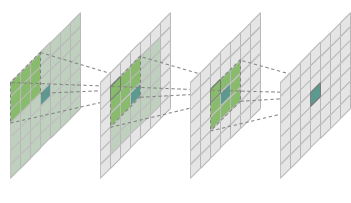
\includegraphics[width=0.7\linewidth]{images/methods_hybrid/field_of_view.png}
    \captionsetup{justification=justified, singlelinecheck=false, width=1\linewidth, labelfont=bf} 
    \caption[]{Figure demonstrating how the use of repeated convolution operations can process global information. The center of the 7x7 grid is marked with ocean color, and it represents an entity in the Lux environment. The increasing field of view is indicated by the shaded green area. The image shows how both local and global information can be utilized in the generation of the entity's action.}
    \label{fig:field_of_view}
\end{figure}

\begin{figure}[htbp]
    \centering
    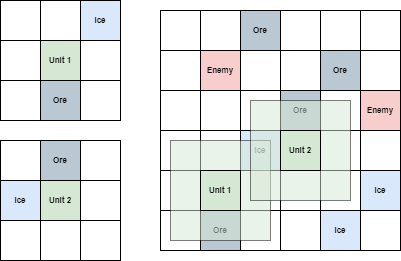
\includegraphics[width=0.7\linewidth]{images/methods_hybrid/feature_extractor/map.png}
    \captionsetup{justification=justified, singlelinecheck=false, width=1\linewidth, labelfont=bf} 
    \caption[]{Image showing how performing shape-preserving convolution operations on the whole observed map (right) is similar to having localized observations for every unit (left). The range of a 3x3 convolution around the units can be seen on the right, marked by an opaque green filter.}
    \label{fig:map}
\end{figure}

\bigskip

\noindent Because a central decision maker is used, but in a way that allows each agent to make their decisions based on their \textbdd{localized observations}, we call this approach \textbdd{hybrid}. Later, we augment this method with the ability to \textbdd{assign rewards to individual} factories and units instead of purely global rewards. This change makes our approach more similar to a truly multi-agent control system while maintaining the benefits of operating with a \textbdd{single global observation} of the game board. We will compare this modified reward-assignment method to the original global reward system. For a more detailed comparison of the mentioned methods, please refer to \autoref{tab:hybrid-table}.

\bigskip

\noindent The training goal remained consistent for this phase as well: \textbdd{learn how to keep factories alive} until the end of the episode. We will now outline the specifications of the training algorithm and model used in the test.

\begin{table}[htbp]
    \centering
    \begin{tabularx}{\linewidth}{Y|C{1.9cm}|C{2.3cm}|C{2.3cm}|C{2.3cm}|C{2.3cm}}
        \toprule
        \textbf{Property} & \textbf{Monolithic} & \textbf{Distributed with Local Observations} & \textbf{Distributed with Global Observations} & \textbf{Hybrid with Global Trajectories} & \textbf{Hybrid with Separate Trajectories} \\
        \midrule
        Passes through Model & once & per agent & per agent & once & once \\
        \midrule
        Observations Stored & once & per agent & per agent & once & once \\
        \midrule
        Observation Size & global & local & global & global & global \\
        \midrule
        Field of View & global & local & global and local & global and local & global and local \\
        \midrule
        Distributed Rewards & no & yes & yes & no & yes \\
        \midrule
        Handles Changing Agent Numbers & yes & no & no & yes & yes \\
        \midrule
        Changing Batch Size & no & no & no & no & yes \\
        \bottomrule
    \end{tabularx}
    \captionsetup{justification=justified, singlelinecheck=false, width=1\linewidth, labelfont=bf} 
    \caption{Table showing the differences between agent control architectures. While storing global observations for every agent with a distributed approach is similar to the hybrid architecture, it requires much more memory and cannot handle changing agent numbers. A hybrid architecture with separating trajectories (\autoref{subsec:grouping}) has every benefit of distributed control.}
    \label{tab:hybrid-table}
\end{table}

\subsection{Environment}

\noindent The environment largely aligns with the description in \autoref{subsec:mono-environment}, with notable changes made to the action space. It now encompasses \textbdd{all actions available} in the Lux AI environment (\autoref{subsec:lux-action}). Additionally, a \textbdd{stricter action masking} mechanism has been applied to limit unnecessary movements and collisions among units.

\subsection{Heuristic Bidding and Factory Placement}

\noindent We retained our initial Gaussian factory placement heuristic outlined in \autoref{subsec:heur-bidding-factory}, making minor adjustments to the weighting calculation and scale of the Gaussian filters to ensure factories are positioned \textbdd{as close as possible to ice}.


\subsection{Actions} \label{subsec:actions}

\noindent Since our goal is to keep the factories alive until the end of the game, we decided to \textbdd{get rid of the lichen mechanic} completely via action masking. This meant that the factories had three possible actions left: build heavy, build light, and do nothing. We forbade the self-destruct action for units since hostility was not needed to achieve the simplified objective.

\bigskip

\noindent Unit actions are comprised of an action type and action settings, depending on the type. Most action settings were implemented heuristically, such as the transfer amount and the repeat flag; however, the most significant parameters were left for the model to decide. Parameters include the move direction, pickup amount, transfer direction, and transfer resource.

\bigskip

\noindent We \textbdd{forbade illegal actions}, such as factory actions that require more resources than the factory's current cargo, moving out of the map, and choosing unit actions that need more power than the agent's current battery. Actions that would slow down exploration were also disabled to \textbdd{speed up the training}. Such actions are doing nothing when the factory could be producing heavy units with its resources, units recharging, or picking up power from factories while at full power. Agent collisions between the team members were also disabled, with keeping track of each unit's movement possibilities and allowing only one at a time to step on a board tile. To stop factories from spawning new units on top of existing ones, agent creation is masked out if a unit is standing on the middle tile of a factory. Agents cannot enter the middle of factories once they have stepped away from them. Actions we considered too complex and unnecessary for the game were also removed with masking, such as picking up resources from factories and transferring resources or power to other agents. The complete list of possible actions and their requirements can be found in \autoref{tab:actions}.

\begin{table}[htbp]
    \centering
    \begin{tabular}{p{1.5cm}|p{3cm}|p{3cm}|p{6cm}}
        \hline
        Entity & Action & Parameters & Requirements \\
        \hline
        Factory & Build Heavy unit & None & - 100 metal in factory \newline - 500 power in factory \newline - middle of factory is empty \\
        \hline
        Factory & Build Light unit & None & - 10 metal in factory \newline - 50 power in factory \newline - middle of factory is empty \\
        \hline
        Factory & Do nothing & None & - no resources to build heavy unit \\
        \hline
        Unit & Do nothing & None & - no power to update action queue \\
        \hline
        Unit & Recharge & Amount [0, 10] & - battery not full \\
        \hline
        Unit & Pickup & Amount [0, 10] & - battery not full \newline - standing on factory \\
        \hline
        Unit & Move & Direction [0, 4] & - no friendly unit at target \newline - enough power \newline - no enemy factory at target \\
        \hline
        Unit & Transfer & Direction [0, 5] \newline Resource [0, 1] & - has cargo \newline - target is factory \\
        \hline
        Unit & Dig & None & - standing on ice, ore or rubble \newline - enough power \\
        \hline
    \end{tabular}
    \caption{Table containing the list of possible actions, along with their requirements. If the requirements are not fulfilled, the action is masked out.}
    \label{tab:actions}
\end{table}


\subsection{Observation}

\noindent We maintained the observation space described in \autoref{subsec:mono-observation}, as it already covered the necessary information for the feature extractor model to align agents for ice resource collection and survivability. Although additional \textbdd{location information} was provided to the network, it was only utilized for \textbdd{auxiliary purposes} and filtering, not incorporated into the forward pass of the feature extractor.

\subsection{Trajectory Separation} \label{subsec:grouping}

\noindent In a \textbdd{multi-agent environment}, where the actions of units and factories are deeply intertwined, the question of \textbdd{credit assignment} naturally arises. Suppose we use rewards corresponding to a global objective or to objectives that require the cooperation of multiple units or factories. In such a scenario, tracking whom to reward and what amount is challenging since multiple agents work towards a common goal. A \textbdd{centralized control} approach offers a potential solution, as all units and factories will belong under a single agent, which receives a \textbdd{global reward} after performing the actions with all entities. Such reward assignment is still possible when using a fully multi-agent approach by giving every agent the sum or mean reward of the team. \label{par:global-rew} However, as we will later see, relying purely on global rewards makes it hard for the model to learn which entity's action was beneficial from the many numbers of entities. The more entities we have, the less of a chance there is that most of them behave optimally. A highly beneficial or determinal action can skew the total reward, which can lead to the \textbdd{reinforcement of bad behavior} or the \textbdd{punishment of good behavior} for the entities whose reward was less dominant in the final sum.

\bigskip

\noindent To tackle this complex problem, we use rewards that can be \textbdd{immediately credited} to the performing or benefiting entity. The ice-dug reward is credited to the performing unit, while the ice-transfer reward is split between the performing unit and the receiving factory. Instead of summing up these rewards to a single global value, we \textbdd{store them separately} to track which entities' actions resulted in how much reward. Since we are using an actor-critic method for training, the critic values should also be distributed. We utilize separate critic value predictions for each entity (\autoref{sec:hybrid-network-actor-critic}). These separate predictions are generated using information about the whole game state, similar to the method of \cite{lowe2020multiagent}.

\bigskip

\noindent In addition to \textbdd{global} and \textbdd{per-entity} reward assignments, we also experimented with putting entities into \textbdd{groups} according to certain grouping rules, where a group's reward is the sum of its members' reward. An example of the reward separations between different groups can be seen in \autoref{fig:rewards}.

\bigskip

\noindent Similar to the rewards and critic values, we also store the action log probabilities and entropies separately. This separation essentially splits every environment step into \textbdd{multiple training examples}, creating multiple \textbdd{distinct trajectories} from the same number of environment steps. The loss calculation does not change from the original PPO algorithm, as the modification simply translates into an additional tensor dimension, and all of the loss samples will get averaged into a single loss value as shown on \autoref{fig:policy-loss}. After the modification, during backpropagation, the weight can be updated more accurately to reinforce good and diminish bad behavior since the fewer number of units and factories that belong to one group, the less of a chance a single entity has of skewing their group's reward, resulting in an inaccurate advantage calculation and a faulty weight update. We will refer to this method as \textbdd{trajectory separation}.

\begin{figure}[htbp]
    \centering
    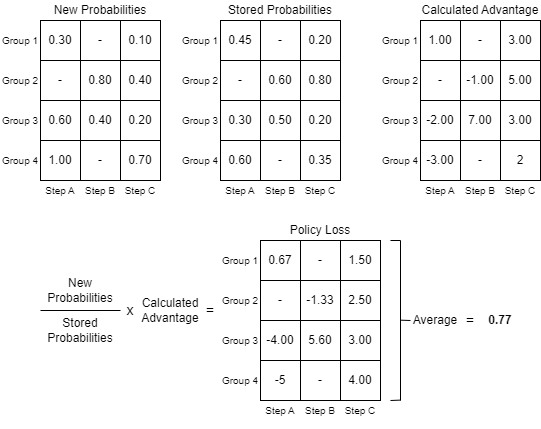
\includegraphics[width=0.7\linewidth]{images/methods_hybrid/trajectory_separation/policy_loss.png}
    \captionsetup{justification=justified, singlelinecheck=false, width=1\linewidth, labelfont=bf} 
    \caption[]{Demonstrating policy loss calculation with the extended dimension. The probabilities and advantages are calculated on a group level. The matrices on the image represent a mini-batch consisting of 3 environment steps. Inactive groups at all steps are marked with a dash, as these are excluded from the training data. The loss gets computed for all active groups, creating more training examples. In the above image, three environment steps resulted in 9 train steps. These loss values are then averaged to get a final scalar loss value. For simplicity, the clipping operation and advantage normalization are left out of this image.}
    \label{fig:policy-loss}
\end{figure}

\begin{figure}[htbp]
    \centering
    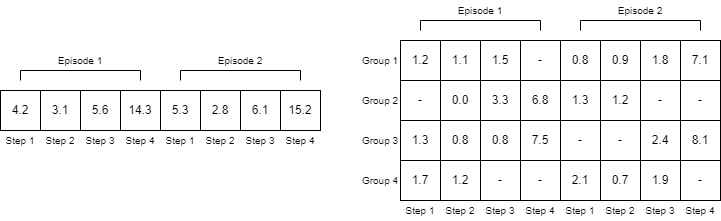
\includegraphics[width=0.8\linewidth]{images/methods_hybrid/trajectory_separation/rewards.png}
    \captionsetup{justification=justified, singlelinecheck=false, width=1\linewidth, labelfont=bf} 
    \caption[]{Image showing the difference between global rewards (left) and rewards distributed into groups (right). The examples are 4-length episodes with random data.}
    \label{fig:rewards}
\end{figure}

\bigskip

\noindent PPO uses a \textbdd{termination flag} stored for every step when calculating future rewards during advantage estimation. This flag signals the start of a new episode and ensures we do not include this episode's rewards in the cumulative return calculation of the previous steps. We need to modify this by adding an \textbdd{extra dimension} to the stored termination flag tensor in order to keep track of the lifecycle of every group since we do not want to calculate steps into the cumulative return where the group was inactive. An example can be seen on \autoref{fig:dones}. A group is marked done when it contains no active units or factories. In the simplest case, when the groups consist of single units and factories, the flag is set to True if the entity: 1. has not been created yet, 2. is destroyed at that step, or 3. remains destroyed. A group consisting of multiple entities can be calculated by performing the AND operation on each of its member's termination flags. At the first step of an episode, every group is marked done.

\begin{figure}[htbp]
    \centering
    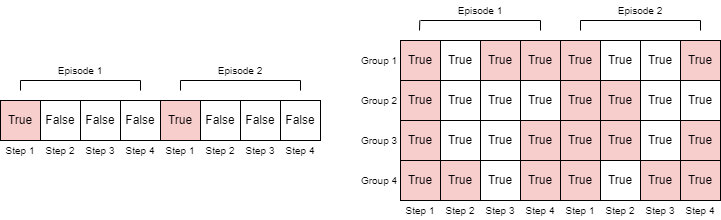
\includegraphics[width=0.8\linewidth]{images/methods_hybrid/trajectory_separation/dones.png}
    \captionsetup{justification=justified, singlelinecheck=false, width=1\linewidth, labelfont=bf} 
    \caption[]{Image showing termination flags for a standard environment (left) and termination flags stored for every group (right). In addition to flagging the end of an episode, the death of a group is also indicated. The examples are 4-length episodes with random data.}
    \label{fig:dones}
\end{figure}


\noindent If we use a grouping rule that allows groups to be occasionally inactive, for example, by assigning every unit or factory to its own group, the number of training examples belonging to one step will \textbdd{not be constant}. Since we divide the \textbdd{mini-batches} by environment step, this could mean that not all mini-batches consist of the same number of training examples. Because the loss values are averaged over a mini-batch to get the final loss, this could mean that training examples that belong to steps with fewer active groups have a \textbdd{more dominant} effect during gradient updates since, on average, they create mini-batches with fewer training examples. Following the same logic, entities at more populated steps of the environment will have \textbdd{less impact} on the final loss. We test using grouping rules that \textbdd{keep group numbers consistent} to overcome this effect. We also experimented with keeping all entity trajectories separate but kept \textbdd{only a set number of training examples} from each step to reduce the training example variance.


\subsection{Feature Extractor Model}
\label{sec:hybrid-network-architecture}

\noindent We use a \textbdd{convolutional neural network} to map the observations into actions for each unit and factory on the board and to output critic values and log probabilities used by the training algorithm. Both the \textbdd{Actor} and \textbdd{Critic} networks have the same \textbdd{Embedding Network} but do not share the weights to avoid the competing objectives of the policy and value functions (\cite{shengyi2022the37implementation}). The structure of the embedding can be seen on \autoref{fig:embedding}. The main building blocks of the network are convolutional layers with \textbdd{3x3 kernels} and padding to \textbdd{keep the board's shape}. The layers alternate between a basic convolutional layer and a \textbdd{residual connection} (\autoref{subsec:residual}), where two convolutional layers are followed by a \textbdd{Squeeze-and-Excitation} block (\autoref{subsec:se}). Each convolutional layer's output goes into a two-dimensional \textbdd{batch normalization} block (\autoref{subsec:batchnorm}), then to a \textbdd{Leaky ReLU} activation function. The weights of the convolutional layers are scaled by their \textbdd{spectral norm} (\autoref{subsec:spectralnorm}).

\begin{figure}[htbp]
    \centering
    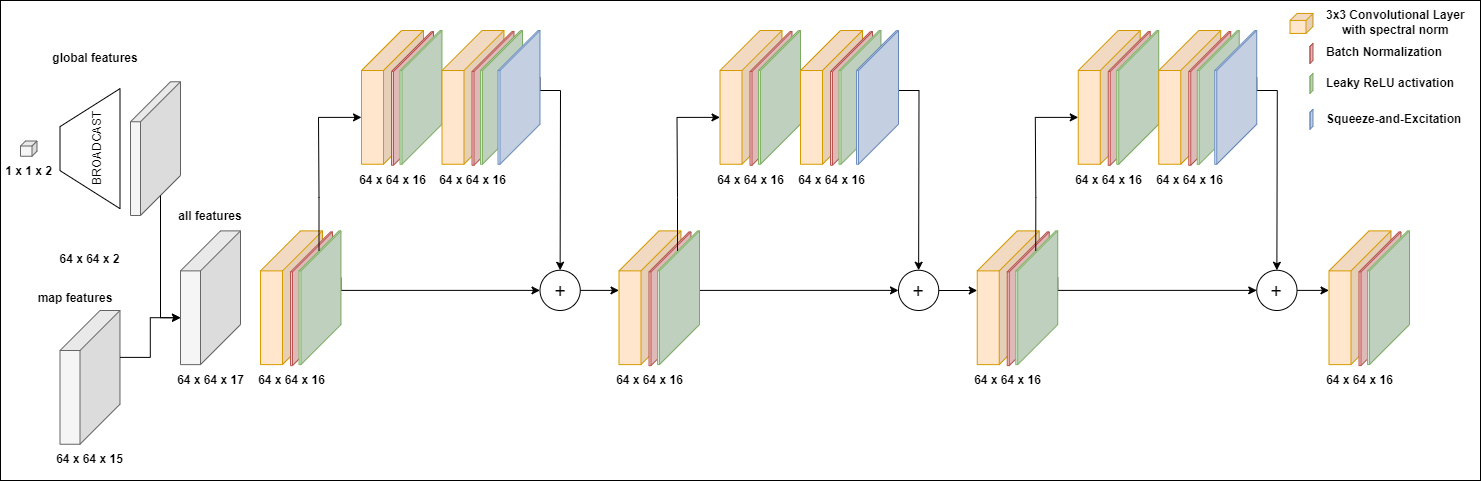
\includegraphics[width=1\linewidth]{images/methods_hybrid/feature_extractor/embedding.png}
    \captionsetup{justification=justified, singlelinecheck=false, width=1\linewidth, labelfont=bf} 
    \caption[]{The structure of the Embedding network. The network uses convolutional layers with 3x3 kernels. Each convolutional block is followed by 2D batch normalization and a Leaky ReLU activation function (\autoref{subsec:leaky-relu}). In order to regularize the network output and allow more layers, we use residual connections with a Squeeze-and-Excitation layer output. This embedding is the backbone of the critic and actor network.}
    \label{fig:embedding}
\end{figure}

\subsection{Actor and Critic}
\label{sec:hybrid-network-actor-critic}

\noindent After the embedding is created from observations, the critic values and the actions are constructed by their respective heads. Since the Lux environment is highly complex, and the entities need to solve multiple tasks in order to reach their goal, multiple reward sources (\autoref{subsec:hyb-rew}) are needed to ensure the rewards are not too sparse for optimal training. In addition to that, since the entities get rewarded based on outcomes, which in reality do not entirely depend on them, it is hard to predict an accurate critic value. Since multiple critic heads already proved to be successful in multi-task environments (\cite{mysore2022multicritic}), we decided to provide a separate critic value prediction for each entity and, in addition to that, provide two additional critic heads for both units and factories, respectively, that use global information for their predictions. The \textbdd{Critic Network} (\autoref{fig:critic}) is made up of 4 components: a \textbdd{unit} and a \textbdd{factory} value network that outputs a value at every board position, and a unit and factory \textbdd{global value} network that, in addition to outputting a value for every position, averages them into a single scalar value. The global unit and factory value scalars are then added to every position of the unit and factory value net output, respectively. This structure ensures that each unit and factory's value calculation is based on \textbdd{both local and global} information. The final outputted values are created by selecting the predicted value at each unit's and factory's position on the board and then adding the value to the entity's group (\autoref{subsec:grouping}).

\bigskip

\begin{figure}[htbp]
    \centering
    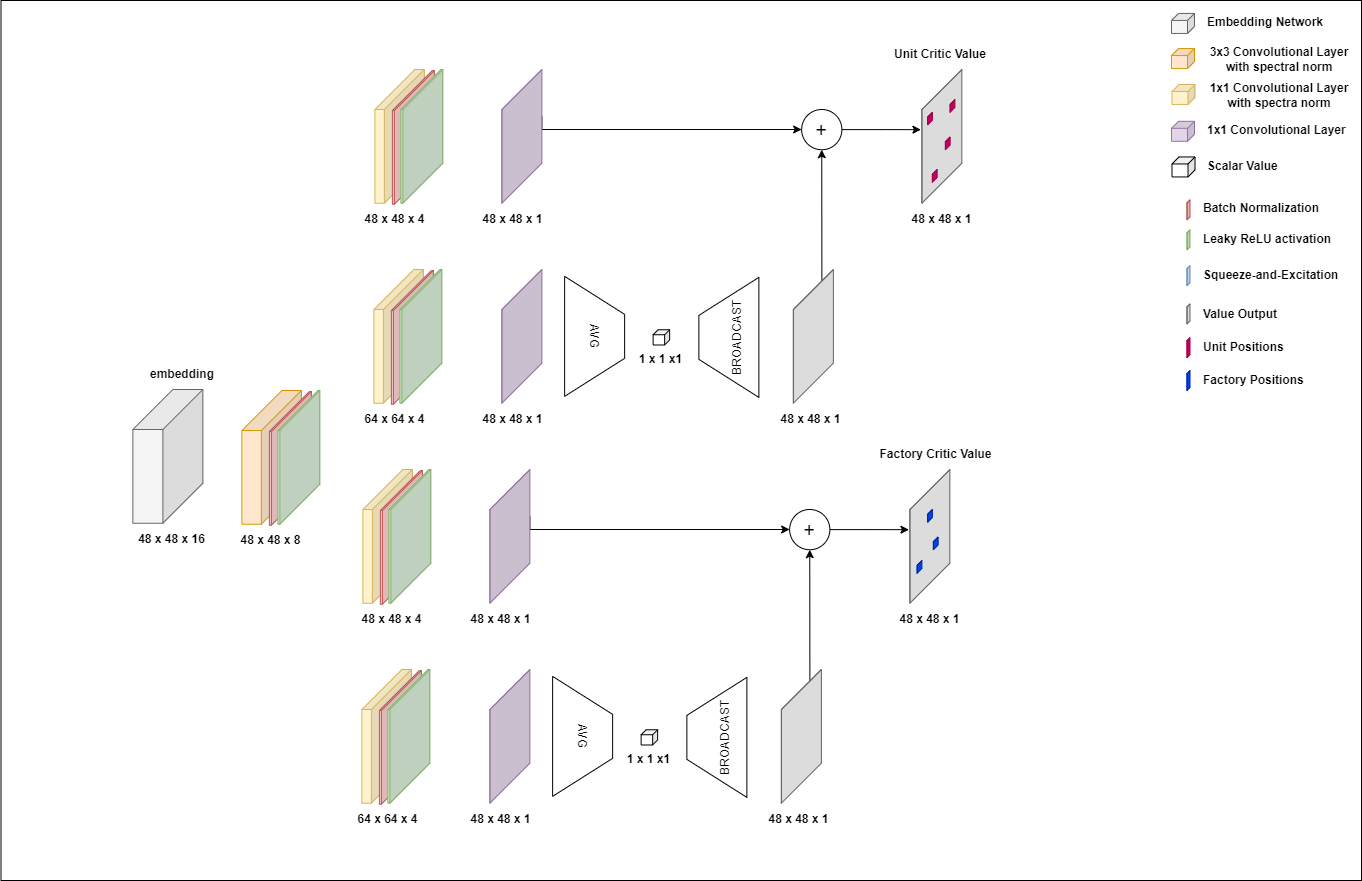
\includegraphics[width=1\linewidth]{images/methods_hybrid/actor_critic/critic.png}
    \captionsetup{justification=justified, singlelinecheck=false, width=1\linewidth, labelfont=bf} 
    \caption[]{The Critic network takes the output of the Embedding and outputs critic values for each entity on the board. Each value is comprised of a local value and a global value, which is averaged over the whole board and then added to each position.}
    \label{fig:critic}
\end{figure}

\noindent Actions are created by the \textbdd{Actor Network} (\autoref{fig:actor}). Factories and units have different action spaces, so different actor heads output their actions. The action space of the factories is a simple discrete action space, while the units have a \textbdd{multi-dimensional action space}, where each action has a different set of parameters. Due to some actions having a \textbdd{heuristic parameterization} (\autoref{subsec:actions}), only four parameter action heads are used in addition to the action type head. The heads output log probabilities, which are then used to create \textbdd{categorical distributions} (\cite{categorical}), discrete probability distributions over the possible actions. Actions are sampled from these distributions after setting the probability of masked-out actions to zero. The sampled actions are outputted in the same board shape at the positions of units and factories. For each entity, the composite action's log probability and the distributions' entropies are summed together at an entity level. These values are added to the total log probability and entropy of the given entity's group (\autoref{subsec:grouping}).

\begin{figure}[htbp]
    \centering
    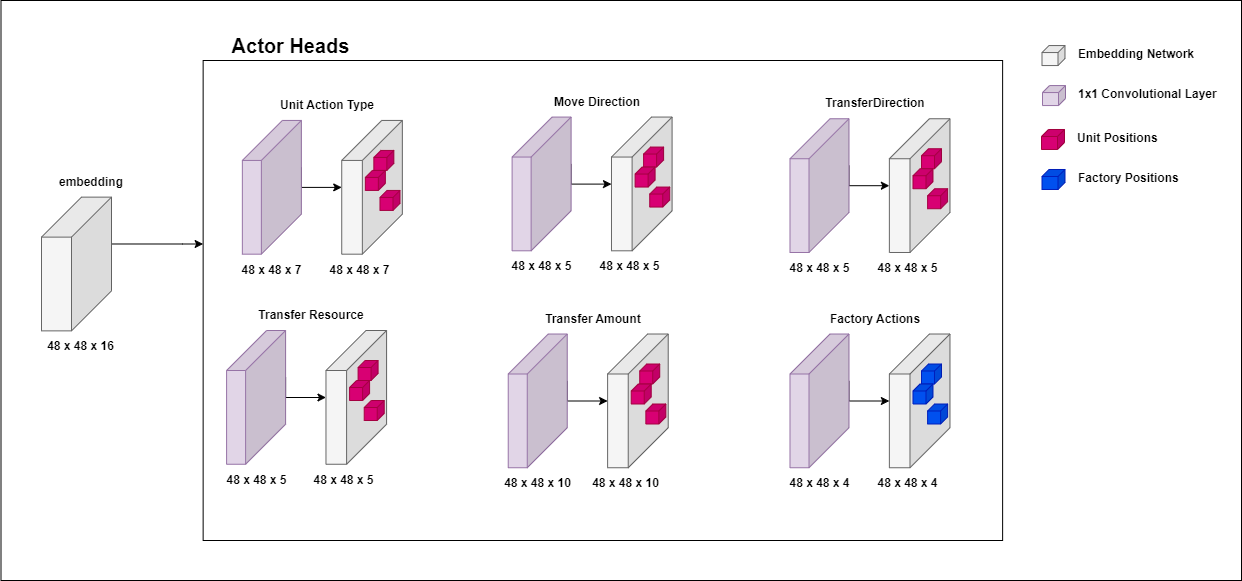
\includegraphics[width=1\linewidth]{images/methods_hybrid/actor_critic/actor.png}
    \captionsetup{justification=justified, singlelinecheck=false, width=1\linewidth, labelfont=bf} 
    \caption[]{The Actor network is made up of separate actor heads, which share the same Embedding network. The output of these heads is the log probabilities of the action distributions. Factory actions have only one output, while unit actions require multiple outputs to parameterize them.}
    \label{fig:actor}
\end{figure}

\subsection{Reward Function}
\label{subsec:hyb-rew}

\noindent The rewards are shaped to \textbdd{encourage the units to bring ice to factories}. In order to achieve this, 1 unit of reward is given after every one water worth of \textbdd{ice is transferred to a factory}. After \textbdd{mining} one water worth of \textbdd{ice}, a 1/10 unit of reward is given to ensure that units find desirable behavior patterns as early as possible. All of these rewards are then divided by to \textbdd{scale them closer to zero}. In order to incentivize units to fill the factories with ice as early as possible, we utilized the same formulation for the multiplication factor in \autoref{eq:reward-early-scaling}.

\subsection{Training}

\noindent To keep experimenting and minimizing training duration, we continued utilizing the Masked PPO algorithm (\autoref{subsec:M-PPO}). Our implementation, derived from \cite{luxai_s2-baseline-source}, provided by the contest organizers as a baseline, \textbdd{differed from conventional approaches}. We opted to train the model twice after each rollout step, using data collected from each player separately. This approach enabled us to gather experience from both players without mixing their training examples during mini-batch creation. Leveraging \textbdd{self-play} and access to both enemy and own player data, we halved our rollout size, which had been doubled in the monolithic approach (\autoref{sec:monolithic-approach-training}), to 4096. Additionally, we reduced the batch size by half, from 1024 to 512. Further details on hyperparameters and subsequent modifications can be found in \autoref{app:c}.

\subsection{Evaluation} \label{sec:hybrid-metrics}

\noindent The evaluation settings remained consistent with those outlined in the monolithic approach (\autoref{sec:monolithic-approach-eval}), employing 12 evaluation environments with episode lengths set to the maximum value of 1024 steps. Transitioning to the hybrid approach allowed us to implement a more \textbdd{comprehensive logging system}, enabling us to devise and calculate more specific training metrics. While episode length serves as a primary metric reflecting our training goal, measuring the \textbdd{amount of ice transferred by units to factories} provides a more nuanced comparison, as it is practically unbounded, unlike episode length, which can be quickly reached in multiple trials. Additionally, we recorded other metrics, such as the \textbdd{average factory count per step}, to assess the ability of entities to maintain multiple functioning factories instead of just one. Most other metrics were retained as baselines for comparison.
